
% Cal Poly Thesis
% 
% based on UC Thesis format
%
% modified by Mark Barry 2/07.
%

\documentclass[12pt]{ucthesis}

\usepackage{ifpdf} 
\newif\ifpdf
\ifx\pdfoutput\undefined
    \pdffalse % we are not running PDFLaTeX
\else
\pdfoutput=1 % we are running PDFLaTeX
\pdftrue \fi

\usepackage{url}
\usepackage{multicol}
\ifpdf

    \usepackage[pdftex]{graphicx}
    % Update title and author below...
    \usepackage[pdftex,plainpages=false,breaklinks=true,colorlinks=true,urlcolor=blue,citecolor=blue,%
                                       linkcolor=blue,bookmarks=true,bookmarksopen=true,%
                                       bookmarksopenlevel=3,pdfstartview=FitV,
                                       pdfauthor={Forrest Reiling},
                                       pdftitle={Extending Windowing Systems to Three Dimensions},
                                       pdfkeywords={thesis, masters, cal poly}
                                       ]{hyperref}
    %Options with pdfstartview are FitV, FitB and FitH
    \pdfcompresslevel=1

\else
    \usepackage{graphicx}
\fi

\usepackage{hyperref}
\hypersetup{
	linktoc=all,
    colorlinks,
    citecolor=black,
    filecolor=black,
    linkcolor=black,
    urlcolor=black
}



\usepackage{titlesec}
% \titleformat{\chapter}[display]% OLD
%     {\normalfont\huge\bfseries}{\chaptertitlename\ \thechapter}{20pt}{\Huge}% OLD
% \titlespacing*{\chapter}{0pt}{50pt}{40pt}% OLD
\titleformat{\chapter}[display]% NEW
    {\normalfont\centering}{\chaptertitlename\ \thechapter}{12pt}{}% NEW
\titlespacing*{\chapter}{0pt}{30pt}{20pt}% NEW

%\titleformat{\section}[block]{first}{label}{12pt}

\titleformat{\section}{}{\thesection}{1em}{}
\titleformat{\subsection}{}{\thesubsection}{1em}{}
\titleformat{\subsubsection}{}{\thesubsubsection}{1em}{}
\titleformat{\paragraph}{}{\theparagraph}{1em}{}

\usepackage[font={}]{caption}

%\renewcommand{\cftchapleader}{\cftdotfill{\cftdotsep}} % for chapters
%\renewcommand{\cftsecleader}{\cftdotfill{\cftdotsep}} 


\usepackage{amssymb}
\usepackage{amsmath}
\usepackage[letterpaper]{geometry}
\usepackage[overload]{textcase}
\usepackage[toc]{appendix}
\renewcommand\appendixtocname{Appendix}

\usepackage{tabularx}
\usepackage{algorithmicx}
\usepackage{algpseudocode}

\usepackage{enumitem}
\setlist{nolistsep}

\usepackage{float}

\floatstyle{boxed}
\restylefloat{table}

\bibliographystyle{abbrv}

\setlength{\parindent}{0.25in} \setlength{\parskip}{6pt}

\geometry{verbose,nohead,tmargin=1in,bmargin=1in,lmargin=1.5in,rmargin=1in}

\setcounter{tocdepth}{4}
\setcounter{secnumdepth}{4}

% Different font in captions (single-spaced, bold) ------------
%\newcommand{\captionfonts}{\small\bf\ssp}
%\newcommand{\captionfonts}{}

\makeatletter  % Allow the use of @ in command names
%\long\def\@makecaption#1#2{%
%  \vskip\abovecaptionskip
%  \sbox\@tempboxa{{\captionfonts #1: #2}}%
%  \ifdim \wd\@tempboxa >\hsize
%    {\captionfonts #1: #2\par}
%  \else
%    \hbox to\hsize{\hfil\box\@tempboxa\hfil}%
%  \fi
%  \vskip\belowcaptionskip}
%\makeatother   % Cancel the effect of \makeatletter
% ---------------------------------------



\begin{document}

% Declarations for Front Matter

% Update fields below!
\title{Juiciness in Citizen Science Computer Games: Analysis of a Prototypical Game}
\author{Eric Buckthal}

\degreemonth{June} \degreeyear{2014} \degree{Master of Science}
\defensemonth{May} \defenseyear{2014}

\numberofmembers{3} 
   \chair{Assistant Professor Zo{\"e} Wood, Ph.D.,\newline Department of Computer Science} 
   \othermemberA{Professor Alex Dekhtyar, Ph.D.,\newline Department of Computer Science} 
   \othermemberB{Assistant Professor Foaad Khosmood, Ph.D.,\newline Department of Computer Science} 

\field{Computer Science} \campus{San Luis Obispo}
\copyrightyears{seven}



\maketitle

\begin{frontmatter}

% Custom made for Cal Poly (by Mark Barry, modified by Andrew Tsui).
\copyrightpage

% Custom made for Cal Poly (by Andrew Tsui).
\committeemembershippage

\begin{abstract}

Incorporating the collective problem-solving skills of non-experts could accelerate the advancement of scientific research. Citizen science games leverage puzzles to present computationally difficult problems to players. Such games typically map the scientific problem to game mechanics and visual feed-back helps players improve their solutions. Like games for entertainment, citizen science games intend to capture and retain player attention. ``Juicy" game design refers to augmented visual feedback systems that give a game personality without modifying fundamental game mechanics. A ``juicy" game feels alive and polished. This thesis explores the use of ``juicy" game design applied to the citizen science genre. We present the results of a user study in its effect on player motivation with a prototypical citizen science game inspired by clustering-based E. coli bacterial strain analysis.

\end{abstract}

%\begin{acknowledgements}

%\end{acknowledgements}

\tableofcontents

\listoftables

\listoffigures

\end{frontmatter}

\pagestyle{plain}

\renewcommand{\baselinestretch}{1.66}


% ------------- Main chapters here --------------------
\chapter{Introduction}
The space we exist in is three dimensional, and this pervades every aspect of our interaction with reality. Everything we touch, see, and hear behaves according to the rules of this three dimensional space and this has made humans exceptionally proficient at reasoning about it, navigating through it, and modelling the behaviour of things within it. Yet when we interact with our computers, an increasingly important part of our everyday lives, most of us do so exclusively through two dimensional user interfaces. 
 
\section{Two Dimensional User Interfaces}

The two dimensional space in which we interact with computers has come to define these interactions in the same way that the three dimensional space in which we exist defines our interaction with reality. We use our fingers or a mouse press 2D buttons and open 2D menus, driving change in the application's 2D interfaces which the windowing system composites into a 2D image to be sent to a 2D display. While this is natural for some intrinsically 2D concepts, like documents and images, other concepts which have no intrinsic spatial embedding, like file systems and networks, are also embedded in 2D when they are presented to the user in order to allow users to reason about them spatially. Even in applications which are intrinsically 3D, like physical simulation and modelling tools, the 3D application space is disjoint from the space in which the user exists (by necessity, since the application has no knowledge of the 3D relationship between the display and the user) and interaction between the 3D application space and the 3D user is traditionally done with 2D input events and 2D images.  

\begin{figure}[ht!]
\centering
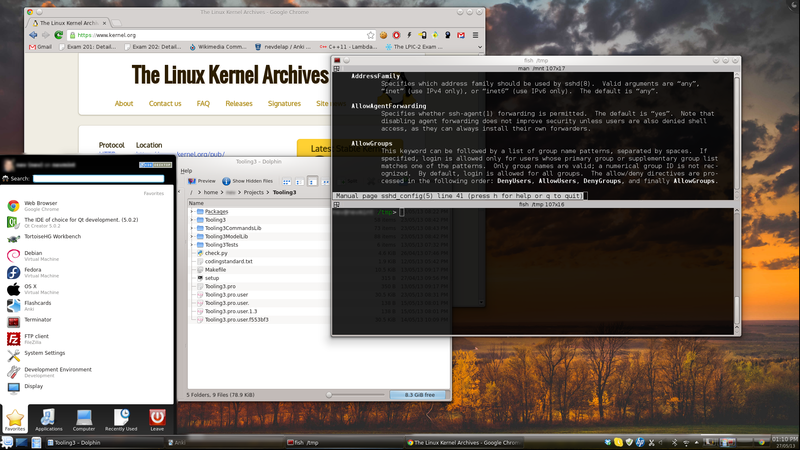
\includegraphics[width=1.0\textwidth]{images/kde.png}
\caption{An example of a typical 2D user interface, showing windows and the desktop environment on a Linux system. Image taken from  \protect\cite{kde-image}}
\label{fig:kde}
\end{figure}
	
The flat nature of contemporary graphical user interfaces has come to define not just the way we interact with applications, but has also become an important factor in the physical design of the computers that run these applications. This is particularly apparent in the mobile computer space, where cost, weight, display power, and mobility concerns push devices toward ever smaller physical profiles, while usability concerns drive the devices toward larger interface surfaces, leading the profile of mobile computers to become flattened against their displays, with the devices acting as a physical embedding of the 2D computer interface within the 3D space in which the computer exists. This forces users to make a tradeoff between the physical profile of their device and the usable size of their interface; larger displays drive up mass both directly and through the need for a larger battery to meet increased power demands, but a smaller displays limit the usable size of the human-computer interface which limits the usability of the device. In desktop computers the same tradeoff must be made, because even absent power and weight concerns the size of the interface is still constrained by the cost of the displays and the physical space needed to mount them in view of the user.

Two dimensional user interfaces are certainly not all bad. There is a natural analog between interacting with documents, images, and folders on a desk and interacting with their digital counterparts on a 2D display (which forms the underpinnings of the familiar desktop metaphor). 2D interfaces also map well onto commercially available display hardware as a result of the two co-evolving for several decades, which keeps the hardware cost of 2D interfaces relatively low. 2D interfaces are mature and well studied, and there is a rich software ecosystem surrounding them which includes sophisticated, full featured user interface toolkits and advanced windowing systems, as well as a broad set of end user applications that provide 2D graphical frontends for almost every task a user need perform on a computer. Users are also familiar with the operation of 2D interfaces, which greatly reduces the time needed for users to learn new applications and improves their productivity with existing applications. 

There are certain applications, like document and photo editing and command line interaction, which fit well with 2D interfaces, and in these applications moving away from 2D interactions would likely be detrimental. However, many applications are intrinsically 3D, or are not intrinsically spatial at all and are embedded in a 2D space because it is simple and well supported, and a transition to 3D interaction has the potential to greatly improve  the usability of such applications \cite{bowman_theory_practice}.

\section{Three Dimensional User Interfaces}

\begin{figure}[ht!]
\centering
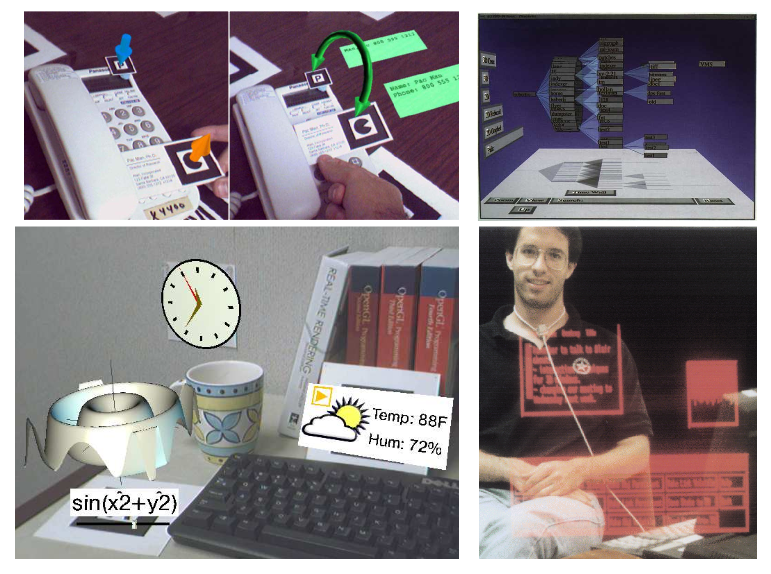
\includegraphics[width=1.0\textwidth]{images/3dui-examples.png}
\caption{Examples of 3D user interfaces. On the left is ARWin \protect\cite{arwin}, on the top right is an example file browser from \protect\cite{info-vis}, on the bottom right is Windows on the World \protect\cite{wotw}}
\label{fig:3dui-example}
\end{figure}

The hardware, software, and theory surrounding high quality 3D human-computer interaction has been the subject of academic research for many decades, and the improved spatial reasoning this provides has been demonstrated to improve usability in a  number of applications  \cite{bowman_theory_practice}. 3D user interfaces are a broad group of interaction paradigms, including everything from desktop 3D modeling with a mouse and keyboard to fully immersive virtual reality.  This thesis focuses on ‘immersive' 3D interfaces, which is used here to refer to 3D interfaces in which the user perceives the 3D interface elements to be in the same 3D space as their body, and has some way of manipulating these interface elements in 3D with corresponding 3D motion by some part of their body.  The hardware needed to support these types of interfaces has traditionally been very expensive, but recent technological improvements in a number of fields have brought many of the core hardware technologies onto the consumer market, bringing both high quality 3D input devices and immersive 3D displays into the reach of everyday computer users.

\subsection{Three Dimensional Input Devices}

Early 3D input devices to come into the consumer 3D interaction market were largely marketed as video game accessories, though their availability has led to their use in a wide variety of other application. These devices can be broadly categorized into two groups: devices which resolve the position and/or orientation of an element held or worn by the user, and range-imaging cameras, which produce a 3D image of a passive scene which contains no sensing elements itself.

\begin{figure}[ht!]
\centering
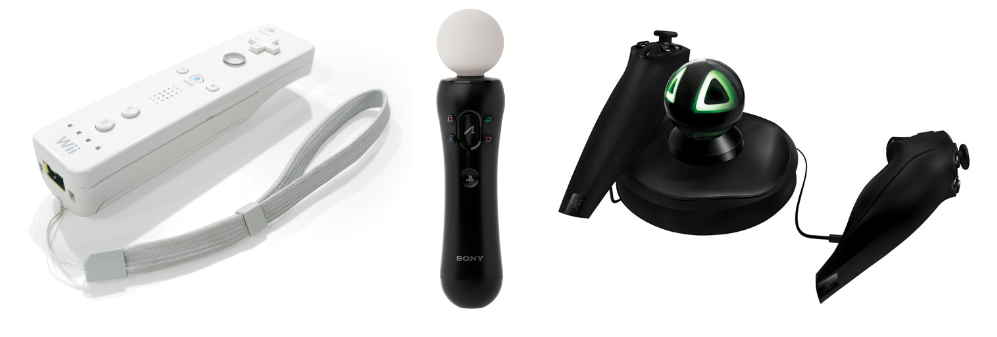
\includegraphics[width=1.0\textwidth]{images/motion-controllers.png}
\caption{From left to right the Wiimote, Playstation Move, and Razer Hydra. Images taken from \protect\cite{wiimote-image}, \protect\cite{ps-move-image}, and \protect\cite{hydra-image}, respectively.}
\label{fig:motion-controllers}
\end{figure}

The first category had its first commercial success in consumer markets in 2006, when Nintendo introduced the Wii Remote, or `Wiimote', as the primary controller for its new Wii entertainment system. This controller, unlike traditional game console controllers, was able to sense its position, orientation, and acceleration along 3 axes. The Wiimote provided limited 3D control within Wii games, and was soon adopted by developers for a wider variety of tasks, including controlling the visualization of volumetric medical data \cite{wiimote-medical} and enabling head tracking 3D on traditional displays \cite{hacking-the-wiimote}. Several devices which provided similar input using a variety of different tracking technologies soon came to market, including Sony's `Playstation Move' in 2009, and the `Razer Hydra' in 2011 (Produced by Sixense Entertainment in partnership with Razer USA). Until the time of this writing all commercially available, consumer grade, 3D tracking solutions have been handheld controllers gripped by the user, but two new multi-sensor, wearable, full-body tracking solutions (Sixense's new magnetic tracking system, STEM, and PrioVR's inertial tracking system) are due to become commercially available within the next year in response to an emerging consumer virtual reality market.
 
Range imaging cameras can be based on a variety of technologies, many of which have been commercially available for many years but have been too expensive to be accessible to a wide body of consumers. In 2009, following advances in real-time structured-light 3D scanning by Primesense Ltd, Microsoft released a range imaging camera based on a Primesense sensor to the public, under the name ‘Kinect', as an accessory for their Xbox 360 game console. Designed to perform full body tracking in 3D on multiple users, the Kinect enabled a variety of new interaction techniques in Xbox games. Like the Wiimote, the Kinect was quickly adopted by third party developers and applied to numerous non-gaming domains, including robotics applications like Simultaneous Location and Mapping \cite{iser-rgbd-slam}, and a variety of medical applications \cite{kinect-medical}. Although the Kinect has received a great deal of attention, being the first consumer grade sensor capable of producing high quality images in real time, many other sensors have since come to market which offer comparable or better performance in a variety of applications and operating conditions. Primesense Ltd., the company that developed the technology underpinning the first generation Kinect, also developed sensors based on the same technology that were released both directly by Primesense under the name Carmine, and through Asus as the Xtion  and Xtion Live, which all offer very similar performance to the first generation Kinect \cite{depth-sensor-comparison}. Very recently, several consumer-grade range imaging cameras have become commercially available which rely on ‘time-of-flight' technology, which has several advantages over structured lighting including lower software overhead, faster response time, and better bright light performance \cite{ti-tof}. This includes Microsoft's next generation Kinect, released with the Xbox One in 2013, and the DS310 and DS325 from Belgium based SoftKinetic. The SoftKinetic DS325, also sold re-branded as the Creative Senz3D, is designed for close interaction and finger tracking rather than full body tracking \cite{softkinetc-products}, and competes in the consumer market with the Leap Motion, a desktop stereo camera designed specifically for hand, finger and stylus tracking in the space immediately above the keyboard. Several other companies, notably Texas Instruments and pmdVision, provide Time of Flight solutions, but to the author's knowledge they do not sell consumer time of flight products as of the time of this writing. 
This is by no means an exhaustive list of 3D input devices; it is meant only to demonstrate the growing diversity of 3D input devices reaching the consumer market, and that this is a relatively recent development. At the surface level, these devices appear to produce a wide variety of input, but when constrained to human-computer interaction applications it becomes apparent that simple input models can capture the useful input produced by all of these devices. Essentially this is because the only mechanism humans have to produce 3D input is the movement of their body through the 3D space or the use of this movement to move an object through 3D space, which can be captured, respectively, by the notions of skeletal tracking and 3D pointing devices \cite{jester}.

\subsection{Immersive Three Dimensional Displays}
\label{sec:3d-display}
	
	The term "3D display" has come to refer to a very broad category of devices, so the term "immersive 3D display" is used here to refer to graphical displays which support both stereo parallax (rendering the scene from a separate viewpoint for each eye) and head-tracking motion parallax (adjusting the position and orientation of these viewpoints based on the 3D relationship between the user and the display), as both are required to create a convincing 3D experience for the user (This is discussed in more detail in the Section~\ref{sec:motion-parallax-and-stereopsis}). This excludes commercial 3D televisions and 3D movie theaters because they do not provide head tracking, and excludes haptic and audio ‘displays' because they are not graphical. There have been many systems which meet these requirements in research and industrial applications, including Responsive Workbenches \cite{responsive-workbench}, Hemispherical Displays \cite{hemi-display}, CAVE Automated Virtual Environments (CAVEs) \cite{cave}, and Head Mounted Displays (HMDs) \cite{sutherland-hmd}, and some of these technologies, particularly CAVEs and HMD's, have received significant research and developments, allowing the technology to mature significantly.
	
\begin{figure}[ht!]
\centering
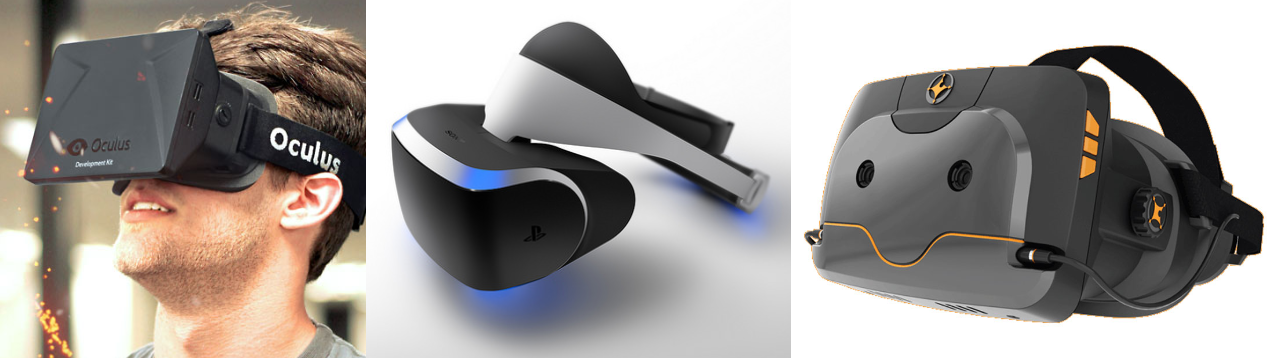
\includegraphics[width=1.0\textwidth]{images/hmds.png}
\caption{From left to right the Oculus Rift DK1, Sony's Project Morpheus, and True Player Gear's Toem. Images taken from \protect\cite{oculus-rift}, \protect\cite{project-morpheus}, and \protect\cite{true-player-gear}, respectively.}
\label{fig:hmds}
\end{figure}
 
Most of these technologies have remained outside of consumer reach, largely due to the large size and high cost of such systems, with the exception of HMDs, whose simplicity and compact design has led them to enjoy intermittent commercial availability for many years. A comprehensive discussion of commercially available HMDs is outside the scope of this paper, but it is worth noting that the recent release of OculusVR's ‘Oculus Rift' development kit to consumer markets has sparked a resurgence in interest in virtual reality for video games and other entertainment applications, leading to the announcement of several new consumer HMDs, including a consumer version of the Oculus Rift \cite{oculus-rift}, Sony's ‘Project Morpheus' \cite{project-morpheus}, and True Player Gear's ‘Totem' \cite{true-player-gear}. 

Priced at only a few hundred dollars, these HMDs put high resolution, wide field-of-view, immersive 3D display technology in the hands of everyday computer users, and the continuing advances of consumer graphics processing hardware gives them the ability to drive convincing 3D scenes onto these displays with commodity hardware. Furthermore, like 3D input devices, the similarity in function between these devices means their behavior can be captured abstractly by relatively simple input and output models. 

\chapter{Background}

\section{Citizen Science}

A citizen scientist is ``a volunteer who collects and/or processes data as part of a scientific enquiry." \cite{silvertown2009new} The roots of citizen science date back to the beginnings of modern scientific exploration, where two centuries ago, science was primarily performed as a hobby \cite{silvertown2009new}. With modern communication and the Internet, the number of potential citizens available to do science has grown drastically. Guidelines for scientific research still apply to citizen science projects: the data collected must be validated, the methods of collecting data must be standardized, and volunteers must receive feedback on their contribution \cite{silvertown2009new}.

Citizen science projects have had remarkable success in advancing scientific knowledge \cite{bonney2009citizen}, especially in the bioscience community. These projects often fall into two categories: obtaining data to study large-scale patterns across nature \cite{bonney2009citizen}, or using citizens ability to analyze researcher-collected data that is computationally expensive \cite{cooper2010challenge} \cite{canthepower} or simply too difficult for computers to complete accurately \cite{milkyway2014}.

\subsection{Games With a Purpose}

There are tasks which are trivial for humans but continue to challenge sophisticated computer programs. Traditional approaches to solving this problem focus on improving artificial intelligence systems \cite{gwap}. ``Games with a purpose" \cite{gwap} advocate the constructive channeling of human brainpower through computer games. The Google Image Labeler \cite{googleimagelabeler} is an example of a game with a purpose where users provide meaningful labels to images on the internet, but the game is also fast-paced and competitive. Many games with a purpose avoid using computer vision techniques that do not work well and instead present players with a form of entertainment. ``People play not because they are personally interested in solving an instance of a computational problem, but because they wish to be entertained." \cite{gwap}

The authors presenting ``games with a purpose" propose that the most important aspect of these games is that they are entertaining \cite{gwap}. Even small changes and modifications of the user interface design could influence the enjoyability of these games. The primary objective of games with a purpose is to generate results, whatever they may be. In game with a purpose, throughput could be defined as the number of game objectives completed per human-hour. Games with a higher throughput should be preferred, but it is important that a game is ``fun" as well \cite{gwap}. No matter how efficiently players can solve a game with a purpose, ``fun" is what convinces players to continue playing.

\section{Games}

\begin{quote}
Games are a nascent and complex medium, one which incorporates many previous forms. A single game might include painting, music, cinematography, writing and animation. If that weren’t enough, video games represent an unprecedented collaboration between creator and consumer. We abdicate authorial control to our players and get … something. We’re not quite sure what yet, but we know that it has potential. To many, interactivity seems to be the most important medium of the 21st century. \cite{swink2009game}
\end{quote}

Video games, like the hardware they exist on, have evolved significantly since their birth. More powerful hardware have engaged players with a complex mixture of audio, video, and tactile experiences \cite{atanasov}. Video games are an interesting medium of expression because they encompass so many aspects from a variety of disciplines. Artist disciplines like graphic design, animation, and sound design are expressed with more technical disciplines like computer graphics and computer science concepts. Unlike specifically broadcast mediums like radio, television, newspaper, or books, video games have an added layer of interactivity \cite{schell2008art}.

Designers of novels, television, and other linear entertainment all stress the importance of user experience \cite{schell2008art}. Readers of novels do not influence the experience of the novel, but the novel instead controls the experience. In video games, the distinction betwen the game itself and the experience is much clearer because there is more control by the player \cite{schell2008art}. The player can control which events happen, the pace of the events, and the randomness they may encounter. Feedback is important in games because it reinforces clues about what effects the player's input have.

\begin{figure}
\centering
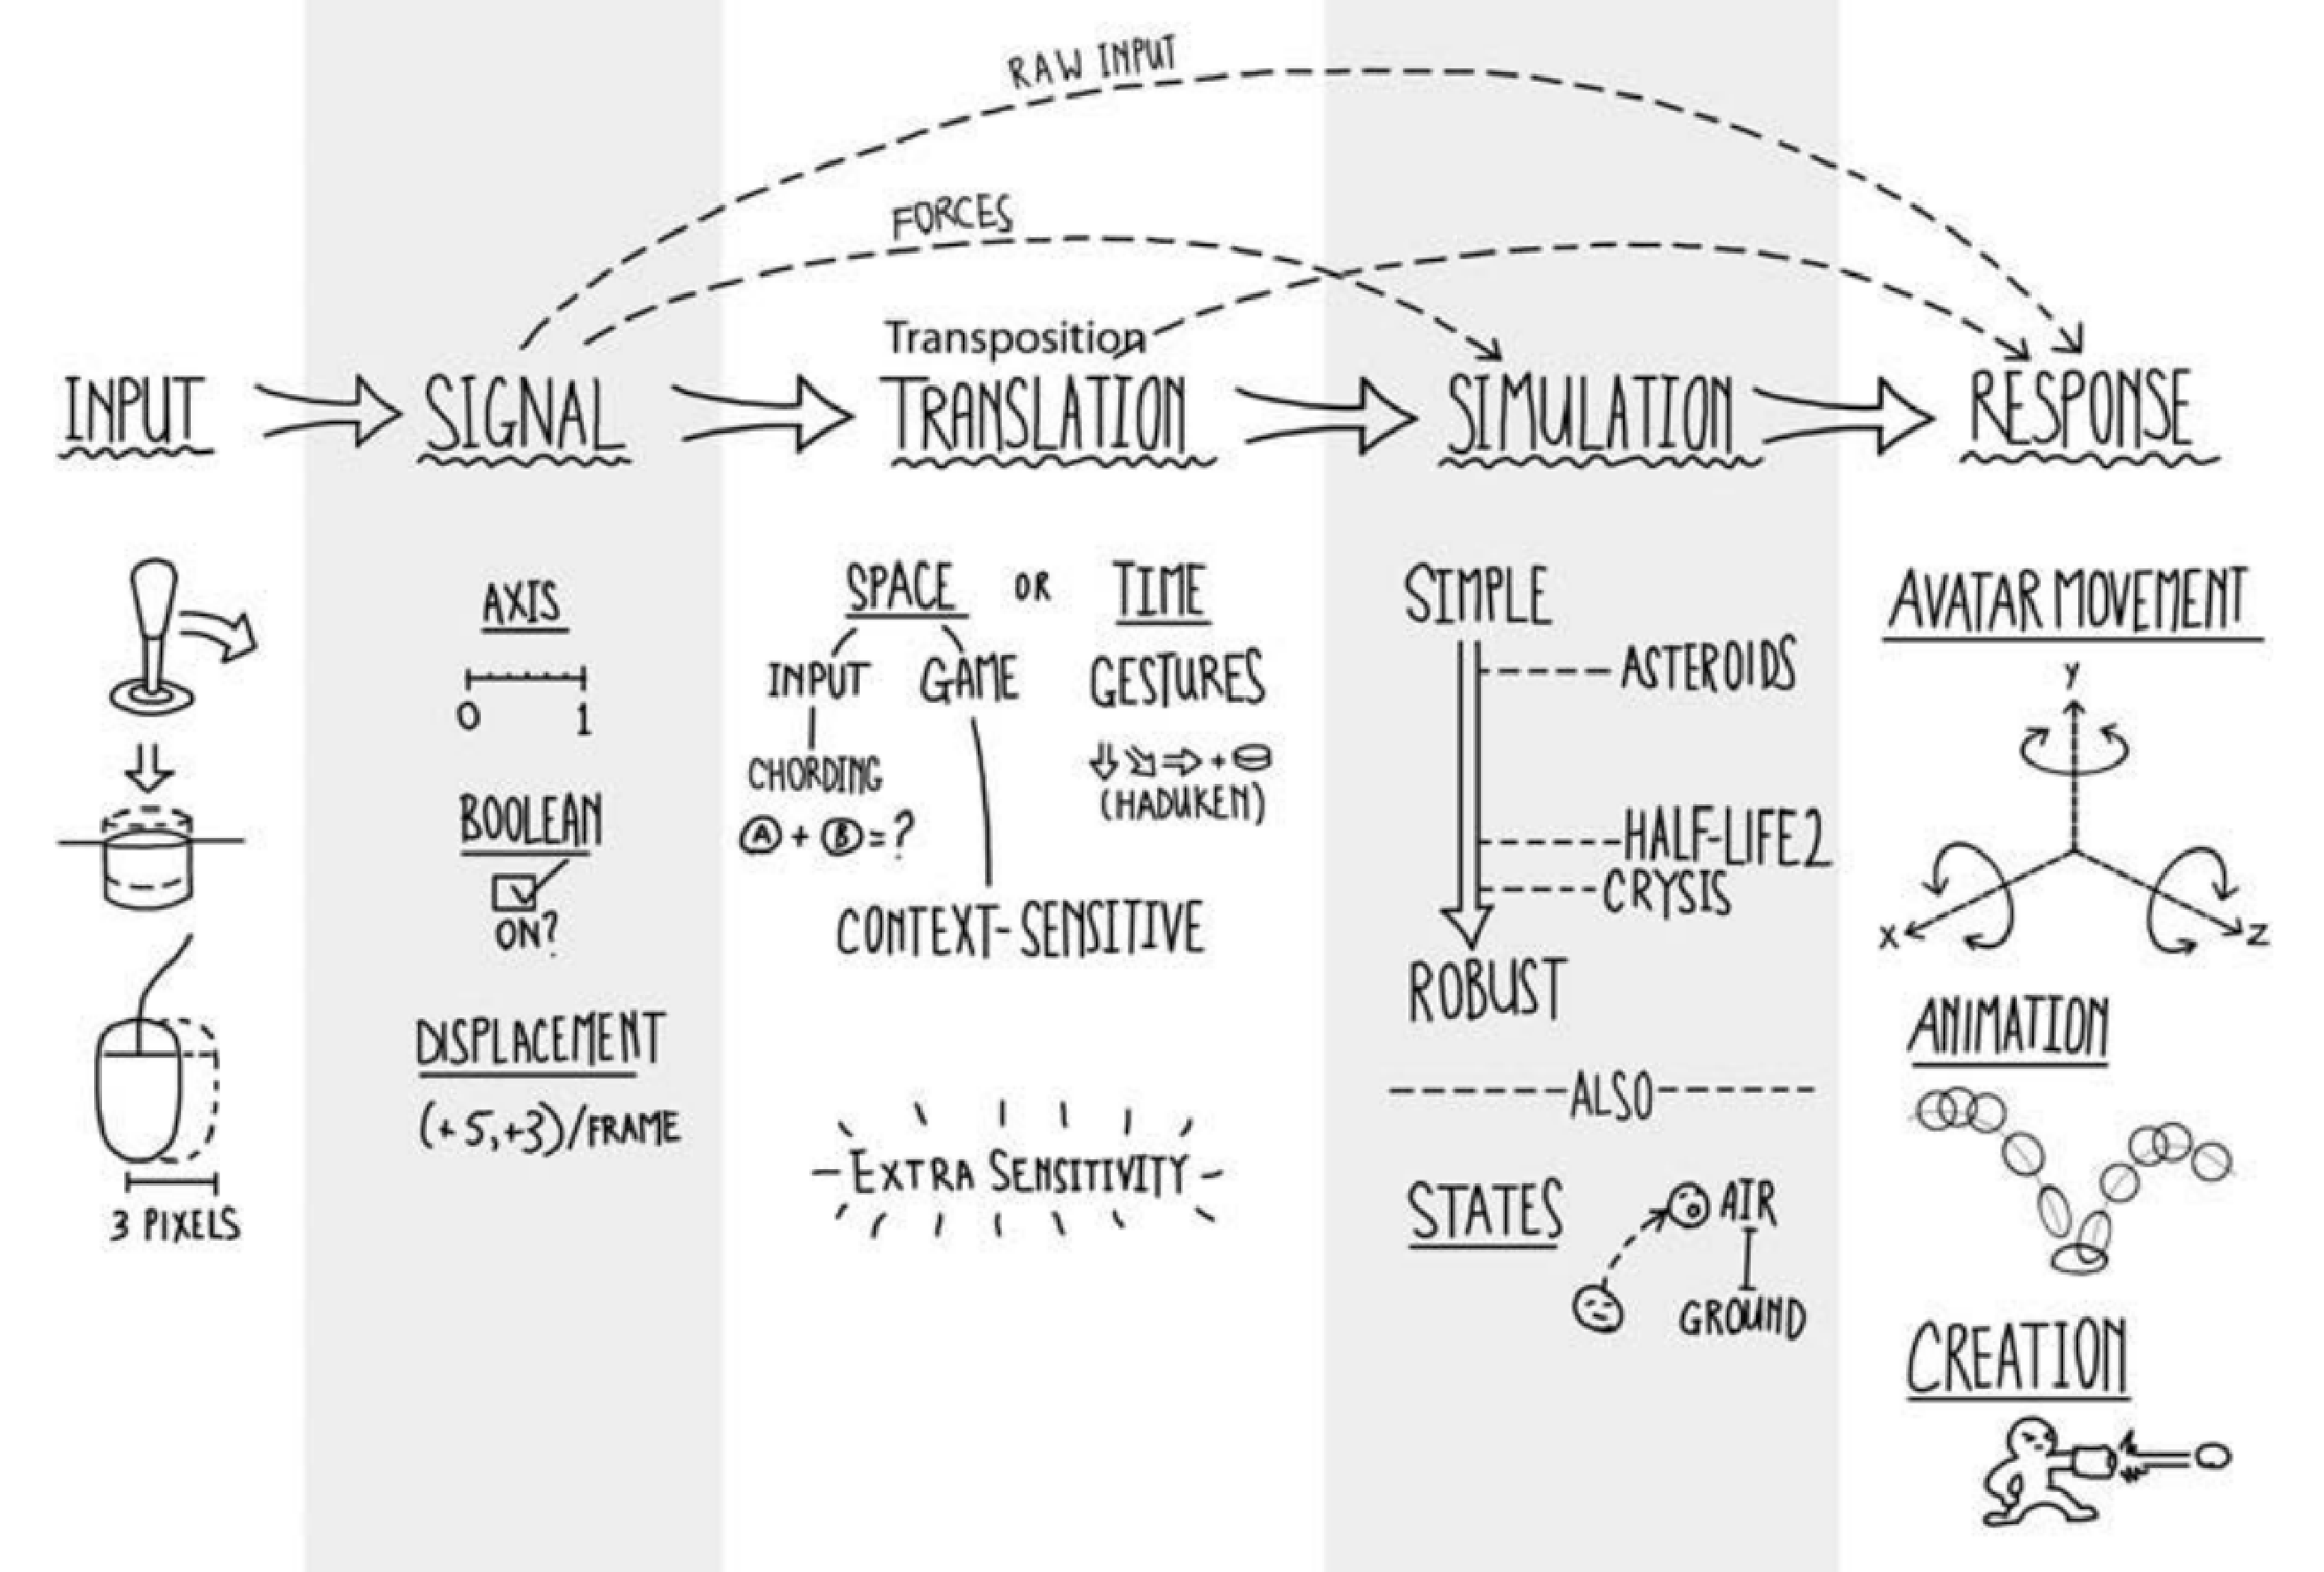
\includegraphics[width=100mm]{images/relationships.pdf}
\caption{The tight relationship between user input and system output is the foundation of great game experience}
\label{fig:relationships}
\end{figure}

While video games are interactive, it's important to note that they, like television or novels, are a tool. They are a means to an experience, Schell is very clear that the experience is completely separate from the game itself \cite{schell2008art}. It is easy to say that the game is the experience because it is real and it exists. The player and game are real, but the experience is imaginary and all games are judged by the quality of this experience because it is the reason that people play games \cite{schell2008art}.

Unfortunately for designers, there is no silver bullet of design. Psychology itself focuses on the measurable, repeatable, controlled results of experimentation but treats the mind as a black box \cite{schell2008art}. There is no objective way to design a game that exhibits a specific experience. Makers of video games (or any entertainment for that matter) can only focus on what seems to be true as opposed to what is definitely true \cite{schell2008art}.

\section{Aesthetics}

``Visceral design is the difference between a high aesthetic design and one that feels infused with soul." \cite{brown2013how} Game and mobile app designers heavily depend on visceral design to create experiences that resonate with the player \cite{brown2013how}. It's about making connections that just ``feel" right. It isn't about just one design choice or mechanic, but a series of overarching interface decisions that acheives a feeling of contentment \cite{brown2013how}. According to the authors, the key to creating visceral design is to focus on feedback loops and essential user flow mechanisms \cite{brown2013how}.

Donald Norman's seminal book, The Design of Everyday Things, proclaims that the most pleasure is attributed to extreme usability \cite{norman2002design}. Later, in Emotional Design, Norman admits that aesthetics create an emotion as essential to the user experience as extreme usability \cite{norman2007emotional}.

Donald Norman breaks aesthetics into three design paradigms: visceral, behavioral, and reflective design \cite{norman2007emotional}. Visceral emotions are the lowest level of emotion--quick judgements that determine whether an experience is good or bad, safe or dangerous. Next, the behavioral level interprets experiences as they happen, whether they are pleasurable and effective. Finally, Reflective emotion is the feeling of self-image and satisfaction that one perceives when remembering an experience. Visceral design can most easily be mapped to appearance, behavioral design to the pleasure and effectiveness of use, and reflective design to the self-image, personal satisfaction, or memories created \cite{norman2007emotional}.

These three designs directly influence human emotion and cognition, which Norman continues to describe as inseperable \cite{norman2007emotional}. Aesthetically pleasing objects enable one to perform better. Scientific studies have again and again refined logical choices and explanations while very few take emotion into account \cite{norman2007emotional}. Norman argues that cognition, the logical, rational side of the brain has equal importance with emotion, or how you feel, how you behave, and how you think. Norman says, ``Emotion makes you smart. Emotion is always passing judgments, presenting you with immediate information about the world. Here is potential danger, there is potential comfort; this is nice, that is bad." \cite{norman2007emotional} The cognitive and the affective sides of the brain work together to determine one's satisfaction of a situation. ``The cognitive side interprets and makes sense of the world around you while emotions allow you to make quick decisions about it." \cite{norman2007emotional}

\section{Game Feel}

``The aesthetic sensation of control is the starting experience of game feel." \cite{swink2009game} This is the pure feeling of enjoying interacting with an interface and having it respond to input---the visceral design component. Experiencing game feel as skill is the process of leanring. This is why some controls feel intuitive and why some control schemes are easier to learn than others.

Game feel is positive feedback from the experience of video games \cite{swink2009game}. Even as game designers, there is no agreed upon defintion for the language to describe game feel. A ``good-feeling" game is one that let's players do what they want without requiring extensive throught process. ``It is to video games what exists in external activities--the aethetics of driving cars, riding bikes, and so on--but nowhere is it so refined, pure, and malleable." \cite{swink2009game}

Game feel is composed from three parts: real-time control, simulated space, and polish \cite{swink2009game}. These ``building blocks of game feel" translate interactions in to experiences. Figure \ref{fig:blocks} demonstrates the connections between these concepts. 

Real-time control is a specific system of interactive where the player intent is transformed into action which the player interprests from the systems output. The user can then percieve the changes and formulate a new action. As players interact with a game in real-time, the correction cycle compares a users actions with the perceptions of changes in the game world. As a player intends to complete an action, they use the games controls and measure the effects to understand how to reach their goal. The correction cycle in figure \ref{fig:correction} separates the levels of intent in real-time control systems \cite{swink2009game}. Though players have a final goal of finding the princess, the correction cycle operates on the level of the avatar moving through the game world. 

Simulated space refers simulated physical interactions in virtual space, perceived actively by the player \cite{swink2009game}. These interactions give meaning and context to the motion and physicality of the objects in space. Players interacting in a simulated space feel that their actions have consequences. They are a frame of reference and gives us the tactile, physical sense of interacting with virtual environments in the same way we interact with our everyday physical spaces. When a player intends to complete an action in the game, a simulated space returns immediate feedback of their action.

Polish refers to the impacts of animations, sounds, particles, and camera shake. These important effects give clues about what type of interaction we are having with game elements and what physical characteristics they are assuming \cite{swink2009game}. Polish is an effect which emphasize or bring clarity to the underlying simulation. Polish effects are only effects that artificially enchance interactions in the game without modifying the underlying simulation and control. Examples are particle effects, crashing sounds as cars collide, camera shake to emphasize a weighty impact. ``This is separate from interactions such as collisions, which feed back into the underlying simulation." \cite{swink2009game}

Many different polish effects can enhance the perception of the game interaction \cite{swink2009game}. ``Juicy" game design borrows heavily from this definition of polish.

\begin{figure}
\centering
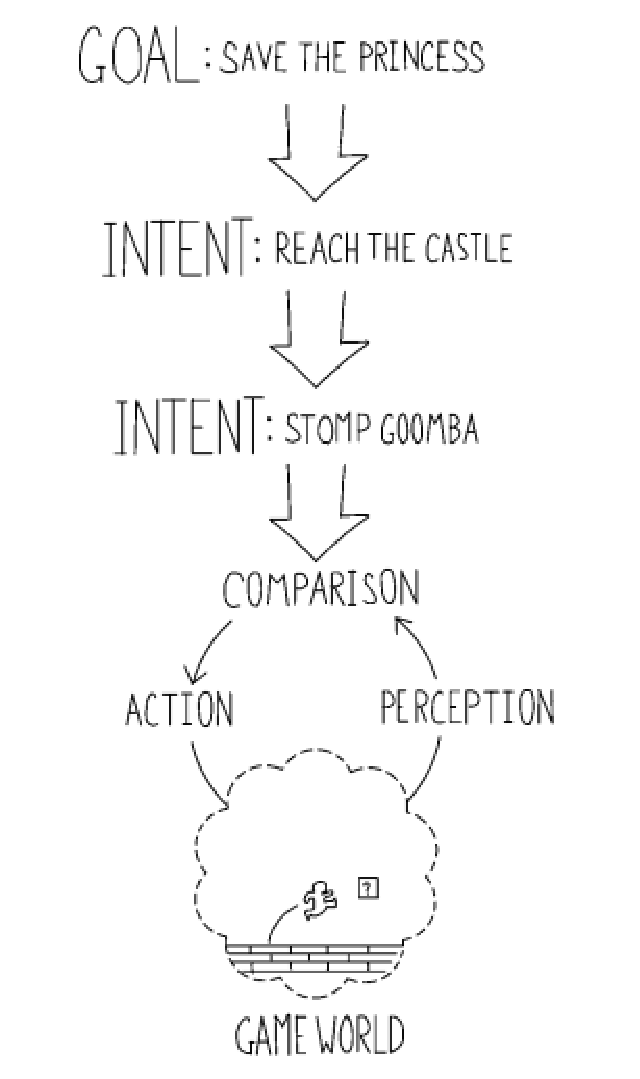
\includegraphics[width=50mm]{images/correction.pdf}
\caption{The correction cycle separates the levels of intent in real-time control systems}
\label{fig:correction}
\end{figure}

\begin{figure}
\centering
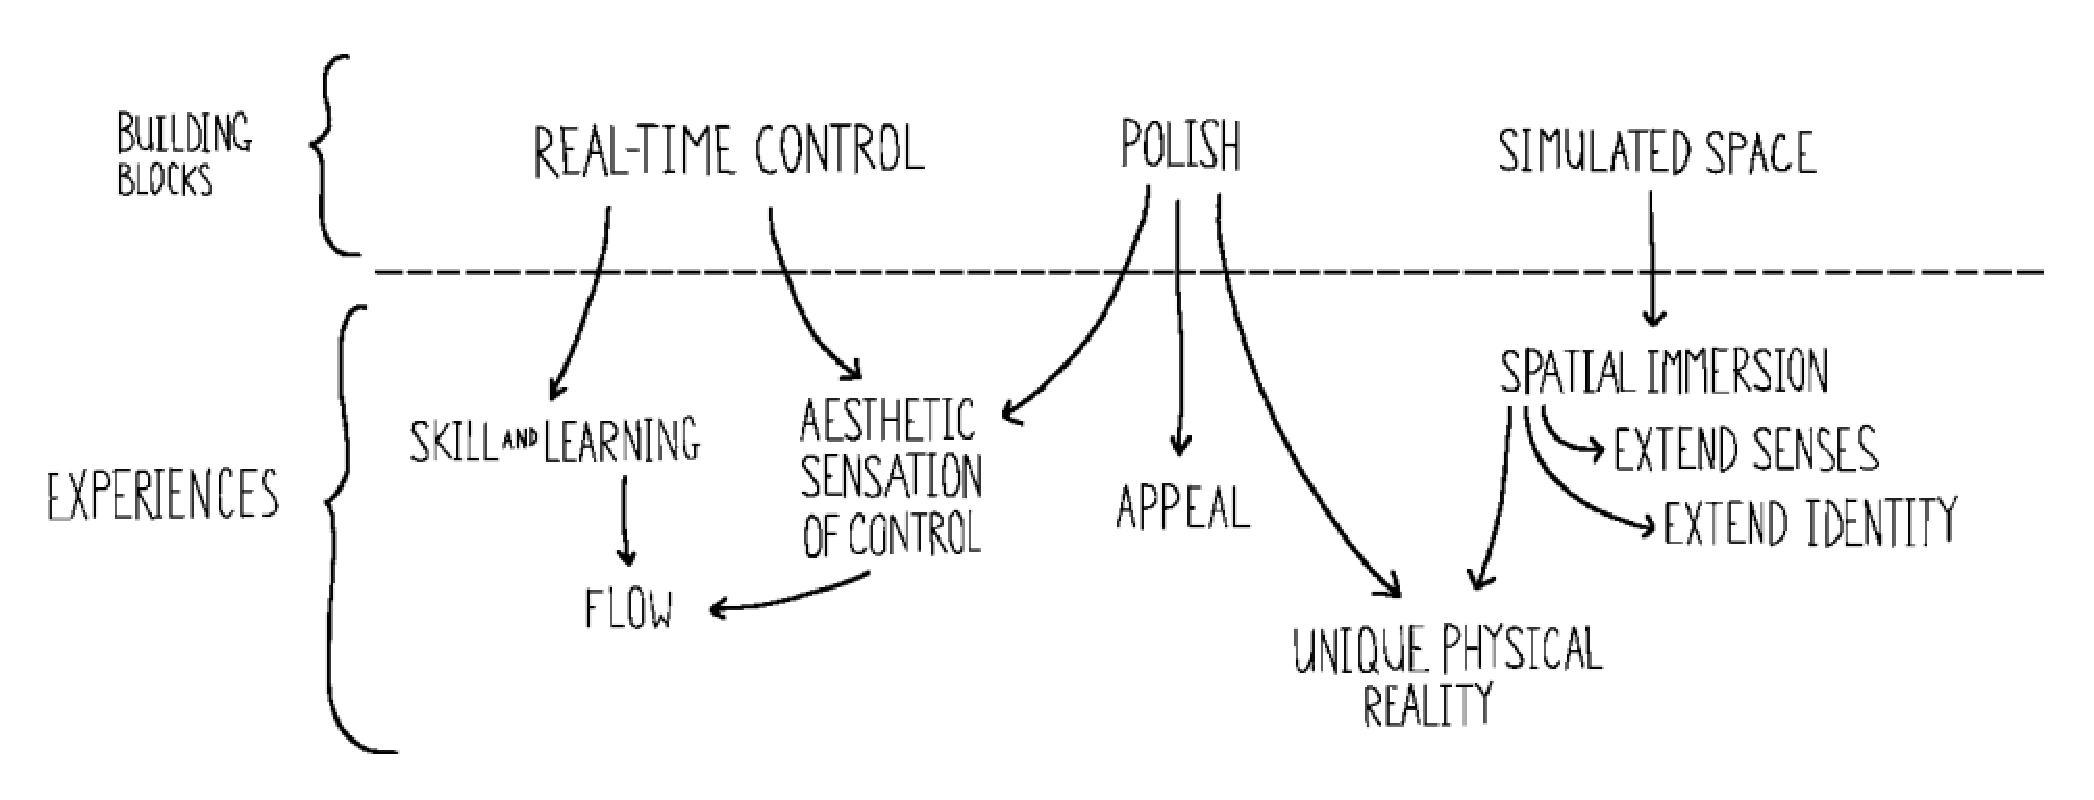
\includegraphics[width=150mm]{images/blocks.pdf}
\caption{Translating game feel into experiences}
\label{fig:blocks}
\end{figure}

\section{Juiciness}

From an influential article published in Gamasutra, ``A `juicy' game feels alive and responds to everything you do--tons of cascading action and response for minimal user input. It makes the user feel powerful and in control of the world, and it coaches them through the rules of the game by constantly letting them know on a per-interaction basis how they are doing." \cite{gamasutra}

The goal of ``juicy" effects is to convey some property about an object or game state by offering feedback clues about how that object interacts with other objects, user input, or its environment. ``Juicy" effects create the difference between a scene of a car starting from stratch and gaining speed and a car screeching and kicking up dust as it speeds away. The car may accelerate at the exact same pace in the two scenarios, but one is loaded with ``juicy" effects that enhance the perception of the experience.

``Juicy" design is aesthetics as much as it is about the experience of playing. Games like Peggle and Bejeweled hark back to the audio-visual bleeps, bloops, flashes of original arcade games, and ``it has to be immediate." \cite{popcap2012} When you're doing well in a ``juicy" game, you don't need to keep your eyes on the score--the game is rewarding you directly through the feedback loop. ``It's not about manipulating behavior, it's about rewarding the stuff that's good for game progress." \cite{popcap2012} A ``juicy" game's appeal doesn't end if when the player reaches the end--simply experiencing the game is fun.

\begin{figure}
\begin{center}
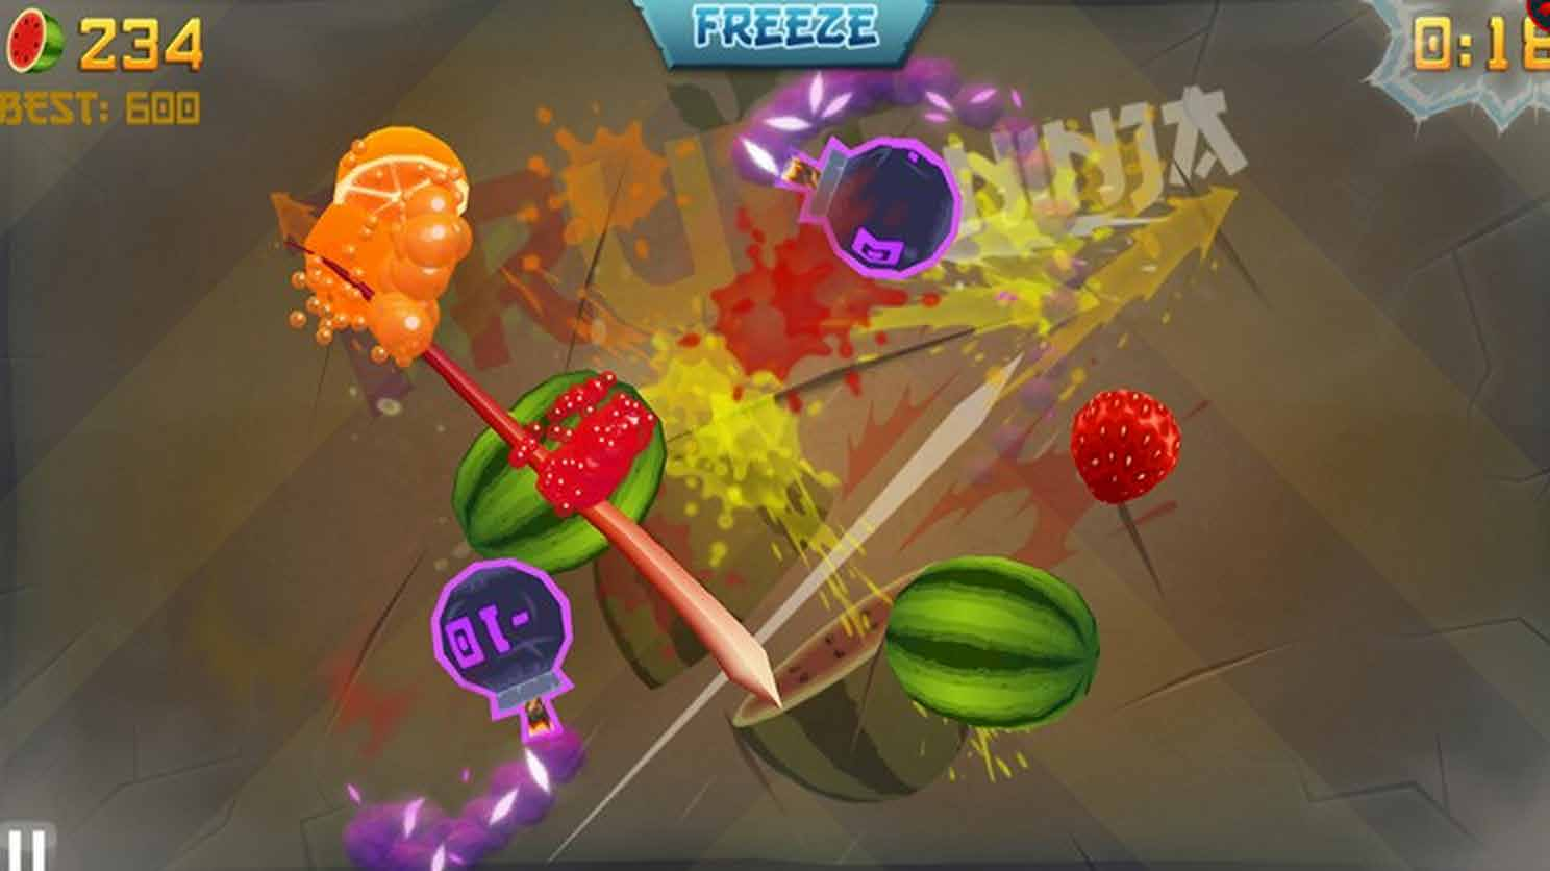
\includegraphics[width=80mm]{images/ninja.pdf}
\caption{With one slice of Fruit Ninja, fruit sections, pulp, juice, and particles all exhibit second order motion}
\label{fig:ninja}
\end{center}
\end{figure}

``Juicy systems reward the player many ways at once. When I give the player a reward, how many ways am I simutaneously rewarding them? Can I find more ways?" \cite{schell2008art} The interface is meant to be more than just a means of communication of information, the interface should be alive, engaging, powerful, and interesting. ``Juicy" interfaces often exhibit plenty of second order motion; that is, motion that is derived from the action of the player." \cite{schell2008art} When you move your finger across the touch-based ``Fruit Ninja", your finger turns into the sharpest knife in the world without a visual representation of a knife. In figure \ref{fig:ninja}, sections of fruit fly in opposite direction and fruit pulp splatters on the wall in a ``juicy" display of second order motion. 

The user deserves to play and explore the possibilites in the ``juicy" interface whereas the ``dry" interface quickly becomes a chore. ``Juiciness" is the combination of satisfaction and empowerment contributing to an overall positive experience \cite{atanasov}.


\subsection{Animation}

\begin{figure}
\begin{center}
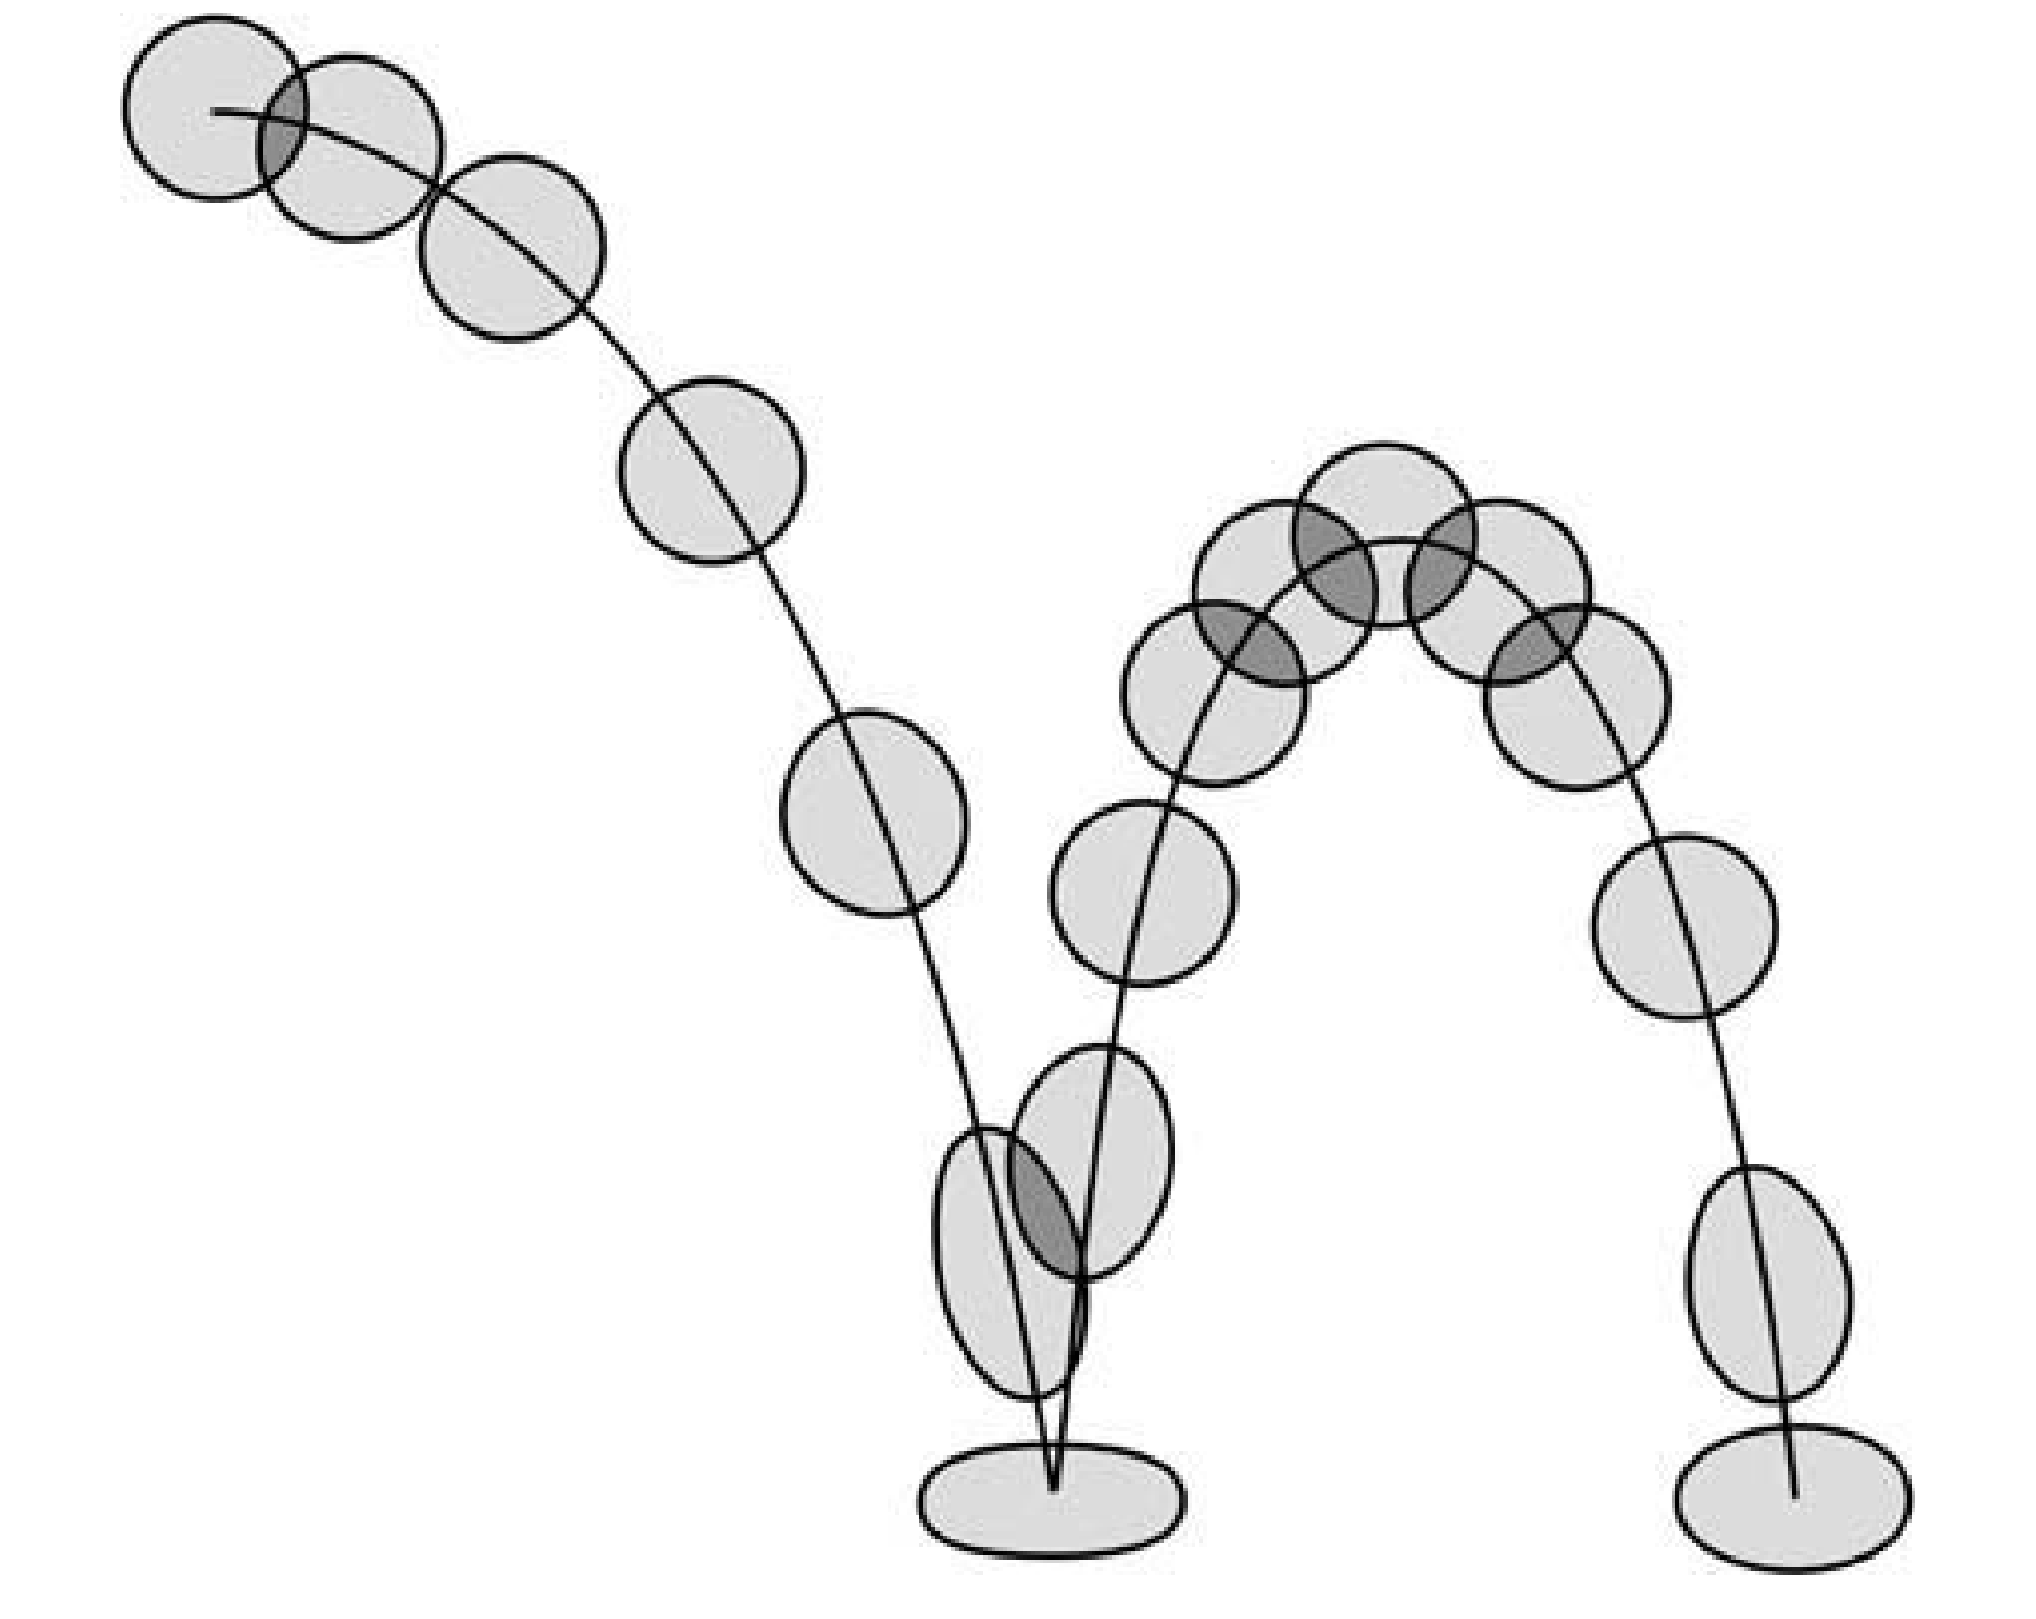
\includegraphics[width=80mm]{images/bounce.pdf}
\caption{The changing shape of the ball as it bounces creates a realistic perception of a bouncing ball, even though the animation doesn’t directly emulate a bouncing ball}
\label{fig:bounce}
\end{center}
\end{figure}

The basic ``principles of animation" were developed by the original animators of Walt Disney Studio, Frank Thomas and Ollie Johnston, during the 1930s \cite{thomas1981disney}. The ``principles of animation" originated the widespread use of concepts like ``squashing and stretching", ``slow in and slow out", ``exaggeration", and ``appeal". 

``Squashing and stretching" gives the illusion of weight and volume to a particular animated effect. It illustrates something fascinating about animation--it is much more believable to exaggerate animations rather than attempting to perfectly replicate real physical properties \cite{swink2009game}. For example, when the bouncing ball animation reaches the ground, viewers are convinced and interested when the ball squishes to almost nothing at the bottom proceeded by stretching when the ball is mid-air. Martin Jonasson uses squashing and stretching as a subtle effect to give life to collisions and interactions in their breakout game \cite{juiceitorloseit}.

\subsubsection{Tweening}

``Slow in and slow out" refers to a specific type of animation that attempts to model accelerations and decelleration. Short for inbetweening, ``tweening" is the process of generating animation frames between two states, giving the appearence of evolution from one state to the next. The process dates back to traditional animation when the head animator would draw the keyframes and have the inbetween frames completed by their assistant. Computer animators use tweening to complete animation between certain desired key frames in animation, or certain states in game design. Tweening is a function of translation over time of a scalar, but vectors can be broken down into multiple scalar values \cite{penner2002robert}. As Martin Jonasson states, ``you can't always use tweening, but it's dirt easy to implement and it feels luxurious." \cite{juiceitorloseit} Most physical scalar values in ``juicy" video games are ``tweened" in some way.

In the physical world, objects infrequently changes states instantly. Whether the change be translation, rotation, colors, or opacity, tweening gives liveliness to motion and make computer elements interesting to watch. Tweening is perfect for game animation because with the quick change of a tweening function, different elements can exhibit completely transitions invoking a different emotional response to its behavior.

\subsection{Visual Effects}

Where animations dictate how objects move in context of their simulated space, visual effects highlight the interaction between objects \cite{swink2009game}. Usually, visual effects appear only momentarily such as sparks flying off the bottom of a car or a crate shattering into an array of splinters. Visual effects can also be caused by an object, though it is not the animation of the object itself. Many sword fighting games employ this effect. A streak of light will follow a sword to emphasize the speed and strength of the character wielding it. In the ``juicy" breakout clone by Martin Jonasson, screen flashes and shaking are used to emphasize the weight of a collision \cite{juiceitorloseit}.

These effects encompass particle effects too. Particle effects are typically temporary indicators of movement or interaction or a specific quality of an item. Smoke and fireworks are common particle creations, and the motion of the particles is much more important than their color or shape. The motion is how players associate meaning with the particles \cite{swink2009game}.

\subsection{Sound Effects}

Sounds effects are repeatable sounds that players can associate with particular interactions in a game. Often a range of sounds will associate with an interaction to keep the players from hearing the exact same sound over and over \cite{swink2009game}.

\chapter{Related Works}
\label{sec:related-works}

Both windowing systems and 3D user interfaces have received a great deal of research over the past few decades, and these fields intersect in a number of ways, so placing this thesis within existing research is somewhat complicated. 

The system described in this paper has the key design goal of being able to seamlessly handle both 2D and 3D interface contexts in the same 3D interface space, so we will compare it to existing research based on this. This primary design goal can be broken down into several secondary goals, including allowing applications to request 2D and 3D windows in the same manner, allowing users to interact with 2D and 3D windows in the same manner, and allowing applications to receive 2D and 3D input in the same manner. Other design goals include allowing applications to use the windowing system without needing to be started by it and allowing 2D applications to window into the 3D space without needing to be modified. To the author's knowledge this set of requirements is not met by any system in existing research.

\section{Two Dimensional Windows in Three Dimensional Environments}
A fair amount of work has been done on managing traditional 2D windows in a 3D space, both in research and, more recently, in production software. These systems can handle multiple 2D windows in a 3D space and can draw the 2D output of a 3D application as a 2D window, but none of them provide a mechanism for unifying the application space with the windowing space for seamless 3D interaction between multiple applications in a single 3D space.

\begin{figure}[ht!]
\centering
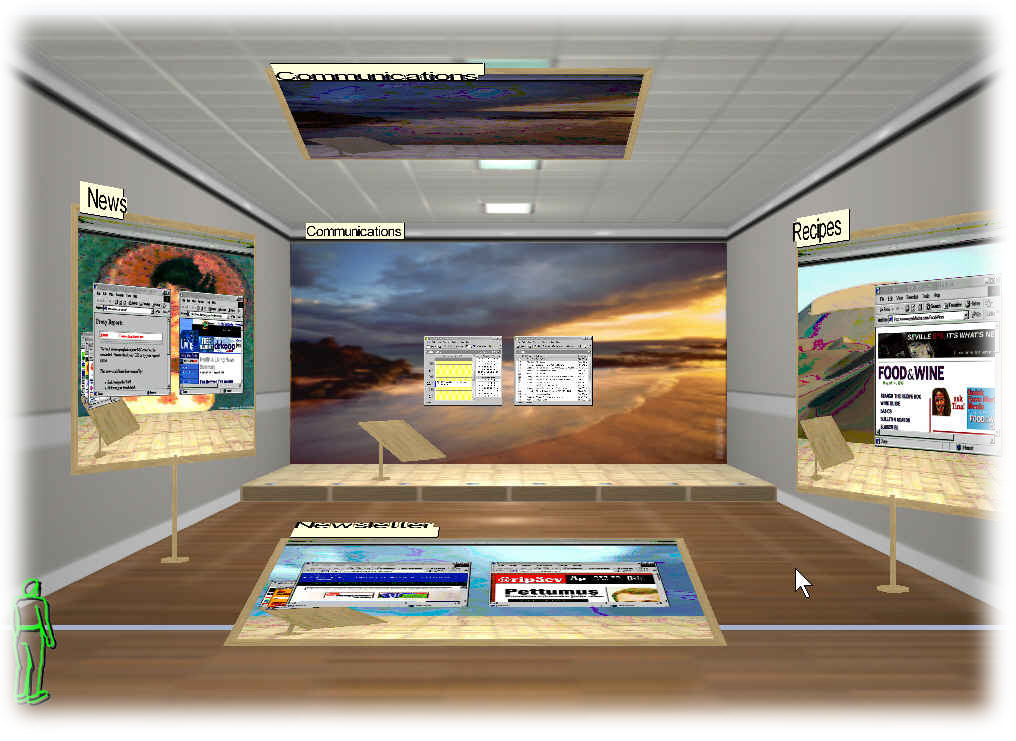
\includegraphics[width=1.0\textwidth]{images/task_gallery.jpg}
\caption{The Task Gallery \protect\cite{task_gallery}}
\end{figure}

The Task Gallery \cite{task_gallery} is a 3D window manager for Microsoft Windows which embeds groups of related windows called 'tasks' into a 3D space to make them appear like artwork hung in a gallery, with the active task on a center 'stage'. This system has some truly 3D user interface elements, like the gallery and the stage, but it exclusively supports 2D windows. 

%\begin{figure}[ht!]
%\centering
%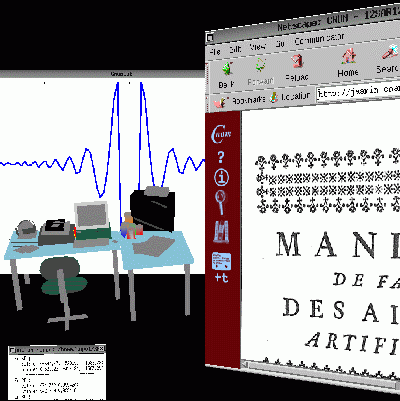
\includegraphics[width=0.5\textwidth]{images/xwindow-immersion.png}
%\caption{Immersion of XWindow applications into a 3D workbench \protect\cite{xwindow_immersion}}
%\end{figure}

Topol describes a system for embedding standard X11 windows into a 3D workspace using techniques similar to those used by modern compositing window managers \cite{xwindow_immersion}. However, like The Task Gallery, this system supports only flat, 2D windows. Additionally, it does not appear that this system support mapping input from the 3D workbench space into the 2D window space.

\begin{figure}[ht!]
\centering
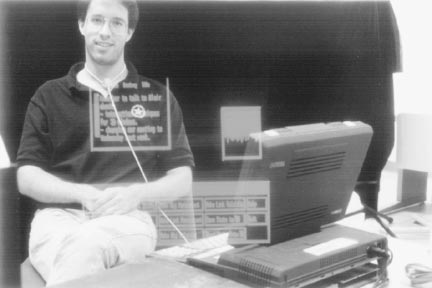
\includegraphics[width=1.0\textwidth]{images/wotw.png}
\caption{Windows on the World \protect\cite{wotw}}
\end{figure}

Feiner et al. demonstrate a similar 3D window management system in an augmented reality setting with their Windows on the World system \cite{wotw}. This system uses a very large X bitmap which applications draw into using traditional means. The display server displays a small portion of this bitmap at a time on a see through head mounted display, and determines which portion of the bitmap to draw into by mapping the pitch and yaw of the user's head onto the x and y coordinates of the bitmap, thereby mapping the bitmap onto a portion of a spherical surface surrounding the users head. Windows can be moved within the bitmap such that they always track the projection of a real world object onto the spherical surface, thereby creating the illusion that the window is attached to that object.
 
\subsection{In Production Software}

As GPU accelerated window compositing has become widely available on consumer hardware (following improved OpenGl support in X.org around 2006) the ability to handle windows in 3D has become broadly available in consumer software.  Some widely used compositing window managers, like Compiz \cite{compiz}, draw window output as textures on 2D surfaces in 3D, allowing them to create compelling 3D visual effects and animate window transitions in 3D space. However, because the architecture of X11 does not give the compositor control of the input system, X11 compositing window managers like Compiz are unable to properly redirect input to the windows while their output is transformed to appear 3D, which seriously limits ability X compositors to create useful 3D interfaces.

\begin{figure}[ht!]
\centering
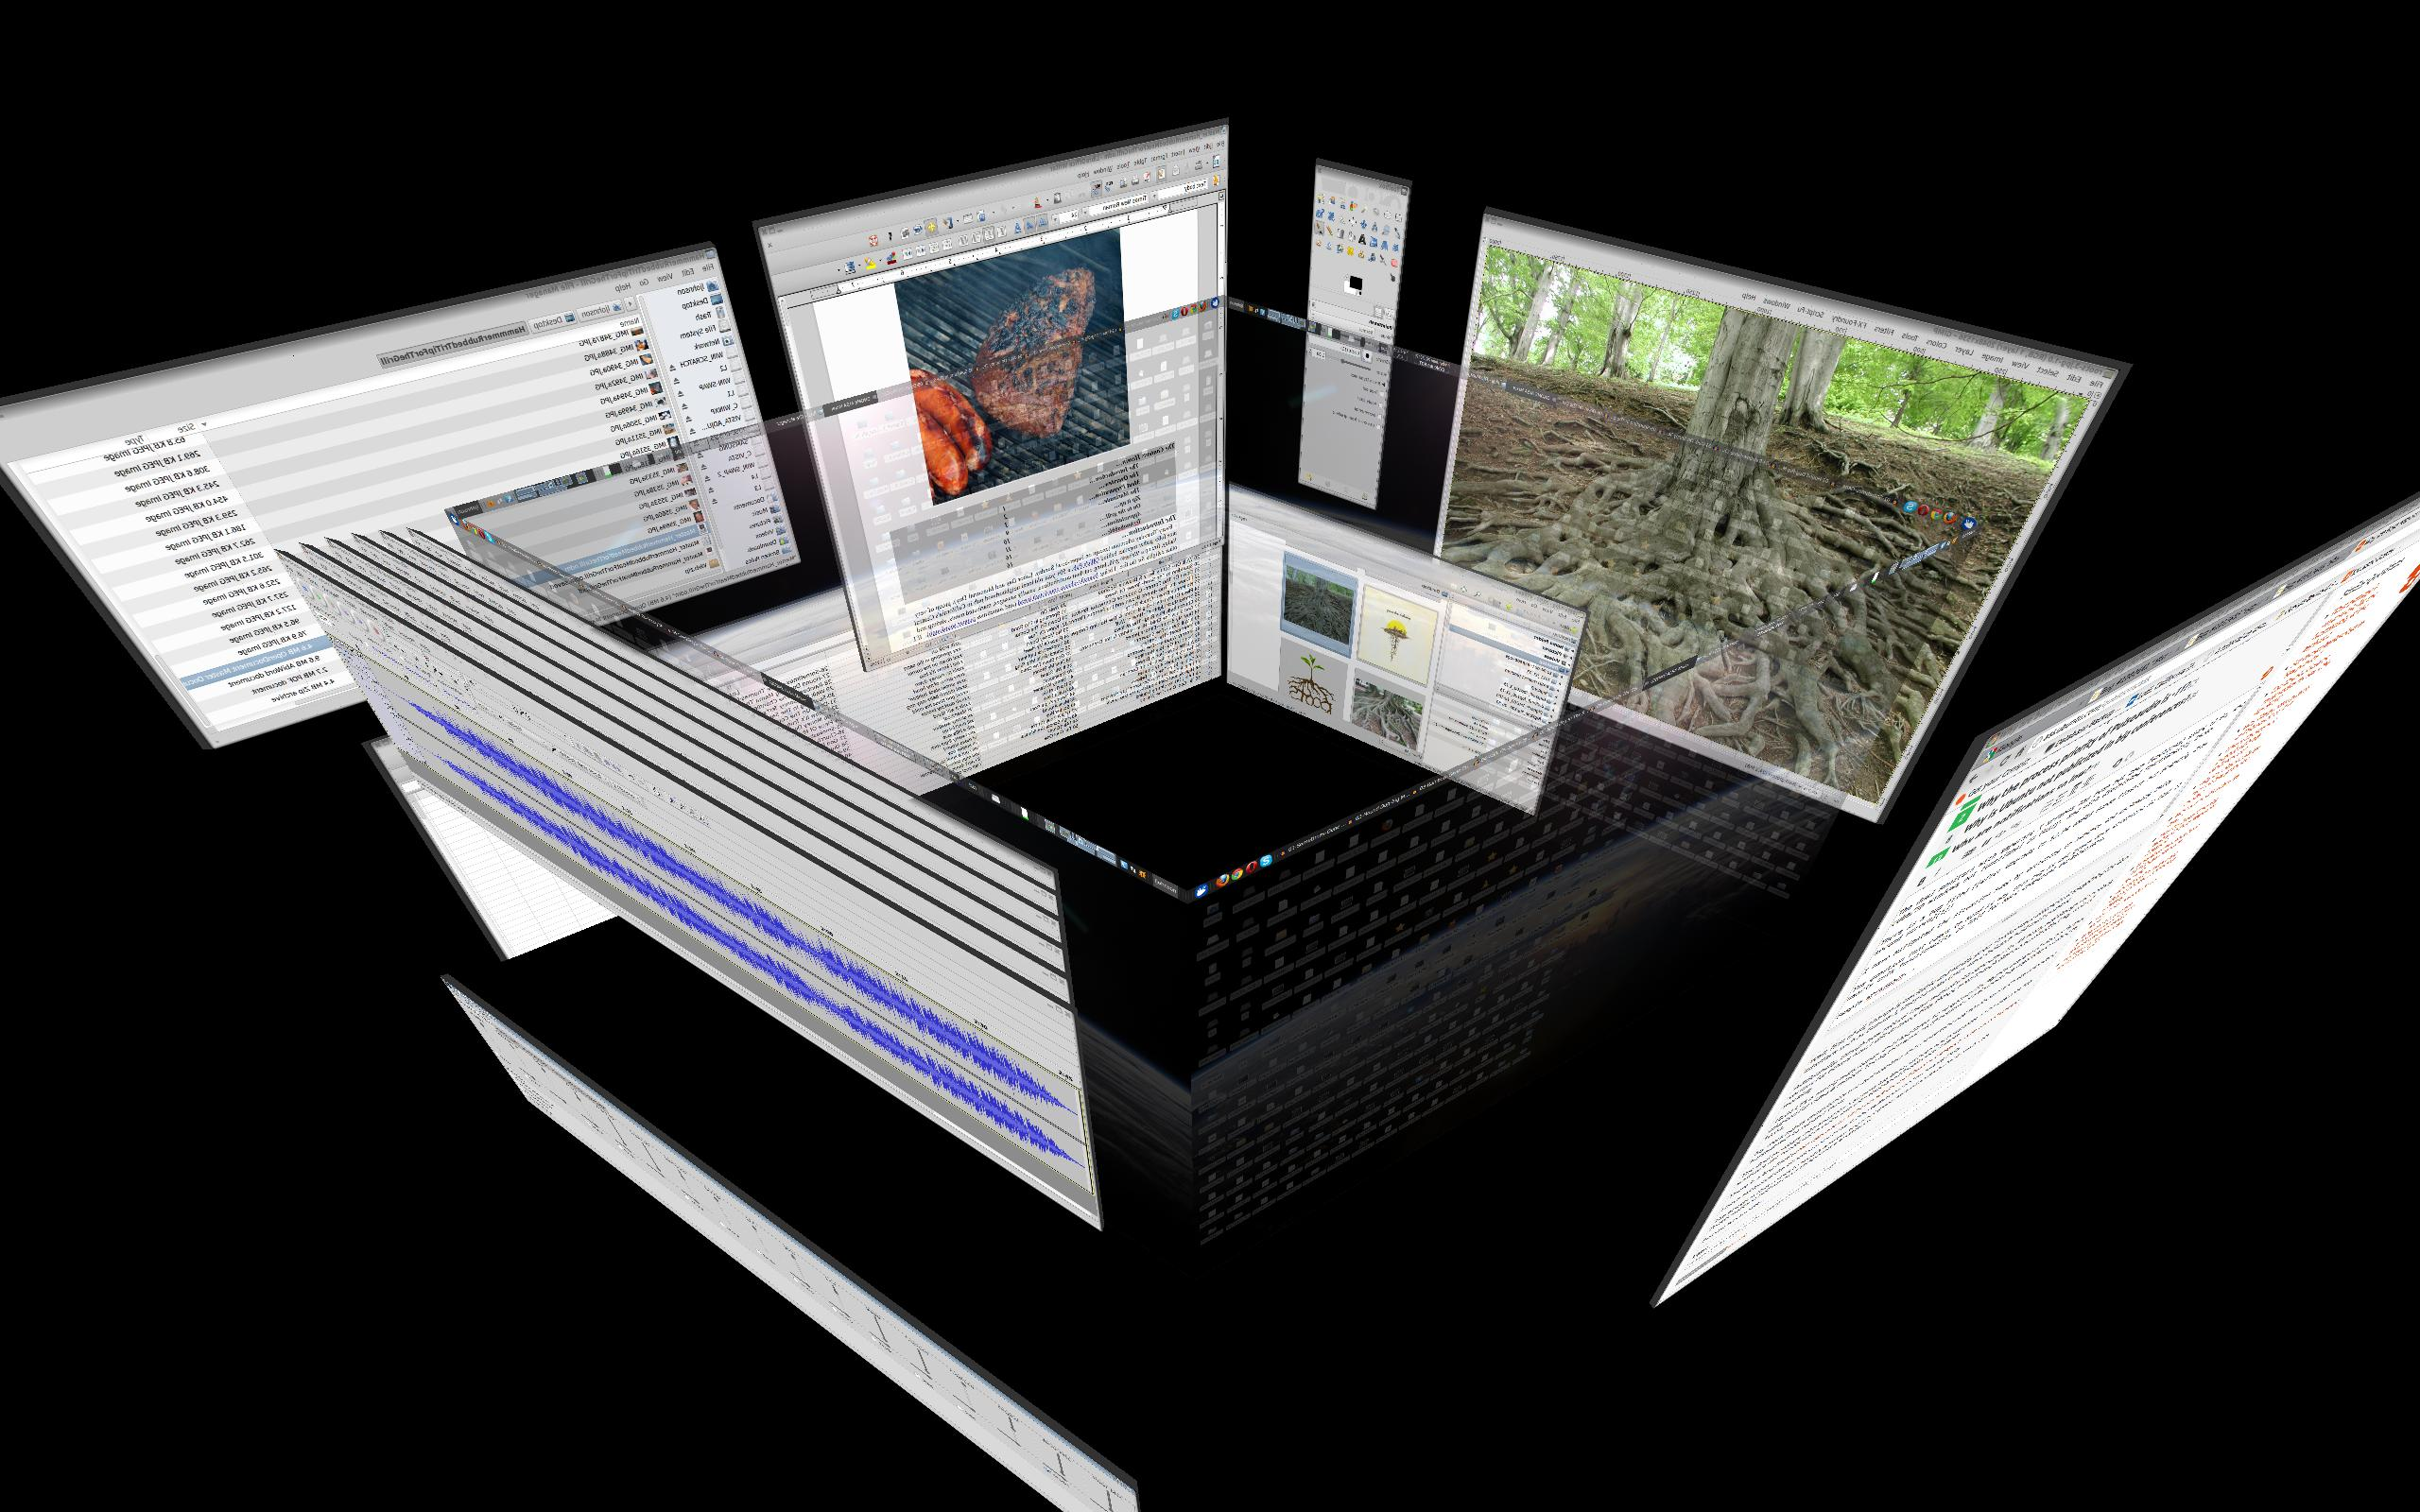
\includegraphics[width=1.0\textwidth]{images/compiz.jpg}
\caption{Compiz Desktop Cube \protect\cite{compiz}}
\end{figure}

The open source community has been seeking to address many of the problems and shortcomings of X11 with the development of a completely new display server protocol called Wayland \cite{wayland}. One of the key differences between Wayland and X is that the display server and the compositor are the same entity, meaning that the compositor can both transform window output to appear embedded in a 3D space while also mapping 3D input back into the 2D window space, allowing traditional 2D windows to be first class citizens of new 3D user interfaces. This, coupled with the simplified architecture of Wayland, is the reason why Wayland forms the basis of the windowing system presented in this thesis.

There are other production windowing systems which allow output from windows to be transformed to appear 3D, used mainly to provide 3D window transition effects like Flip 3D in Windows Vista and Windows 7. To the author's knowledge no production window manager allows normal window interaction while the windows' output is transformed to appear 3D.

\section{Three Dimensional Windows}

There are systems in existing research which explore concepts similar to the 3D windows described in this paper. For the most part what separates them from the work in this thesis is lack of support for windowing by external applications, limitations on what clients are allowed to draw within their windowing volumes, or lack of first class support for 2D windows.

\begin{figure}[ht!]
\centering
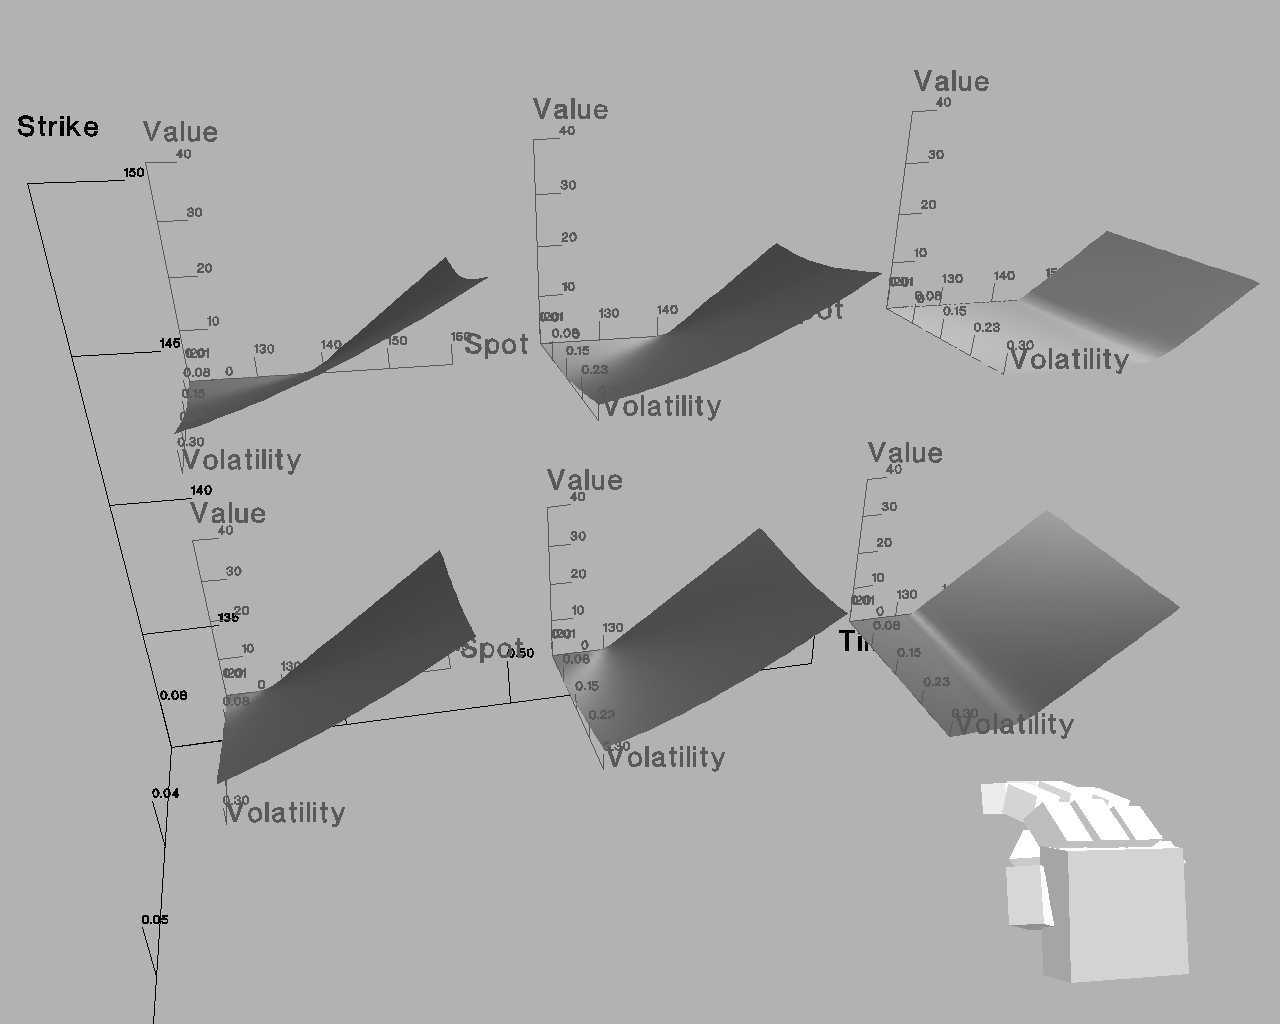
\includegraphics[width=1.0\textwidth]{images/n-vision.png}
\caption{The n-Vision Test Bed \protect\cite{nvision}}
\end{figure}

The earliest work (to the author's knowledge) which explores such a concept is Feiner and Besher's n-Vision testbed \cite{nvision} in 1990, a system designed to facilitate the visualization of high dimensional data using a hierarchy of nested 3D visualization volumes called 'boxes'. Each box draws a 3D slice of the multidimensional space by mapping the high dimensional function across 2 selected independent variables within the box, with all other independent variables held fixed within the box at a value determined by the box's position within its parent box. This nested hierarchy of boxes is much like a 3D analogue of the X protocol's hierarchy of 2D rectilinear windows (as the authors note), but it is not designed to allow third party applications to create such volumes and draw content inside of them. It also lacks support for 2D windows, and the capabilities of the system appear to be limited to graphing multivariate functions.

\begin{figure}[ht!]
\centering
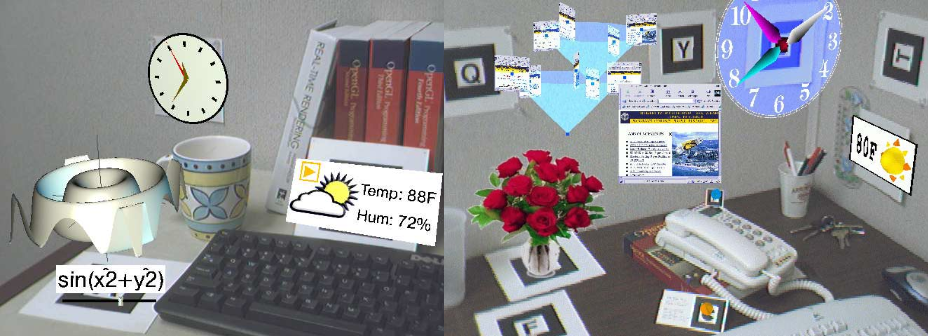
\includegraphics[width=1.0\textwidth]{images/arwin.png}
\caption{Example ARWin Desktops \protect\cite{anywhere-augmentation}\protect\cite{arwin}. Note the function graph and bouquet programs, which draw 3D content into the 3D interface space.}
\end{figure}

DiVerdi demonstrates a 3D augmented reality window manager called ARWin \cite{arwin} which he uses to manage 3D user interface elements and 2D windows in his Anywhere Augmentation system \cite{anywhere-augmentation}. It is difficult to firmly compare this thesis to ARWin because the description of ARWin does not go into great detail about the system's implementation. One difference that is clear is that the system lacks native support for 2D windows, instead supporting 2D windows through a VNC client which outputs the windows content to a texture (which limits 2D support to applications without hard latency requirements). While their system supports multiple applications drawing 3D user interface elements in the same 3D space, it is not clear what constraints are imposed on this process or the mechanism by which 3D applications draw content in the 3D space. It is also unclear how applications request a session with the display manager, and even if this is possible without the display manager starting the application itself. No documentation regarding the windowing mechanism could be found. 

\section{The Three Dimensional Workspace Manager (3DWM)}

The system in existing research which appears to be the closest thing to the system described in this thesis is 3DWM \cite{3dwm}, a system designed to provide a network transparent hardware abstraction layer for 3D user interfaces and a reusable 3DUI toolkit to ease the development and research of new 3D user interfaces. Like the system described in this thesis (and like the X Window Protocol and the Wayland display server protocol) the basic system architecture consists of a display server which manages the input and output hardware, and a set of independent client applications which are able to request that the display server notify them of input events and draw content for them on the output hardware. 

\begin{figure}[ht!]
\centering
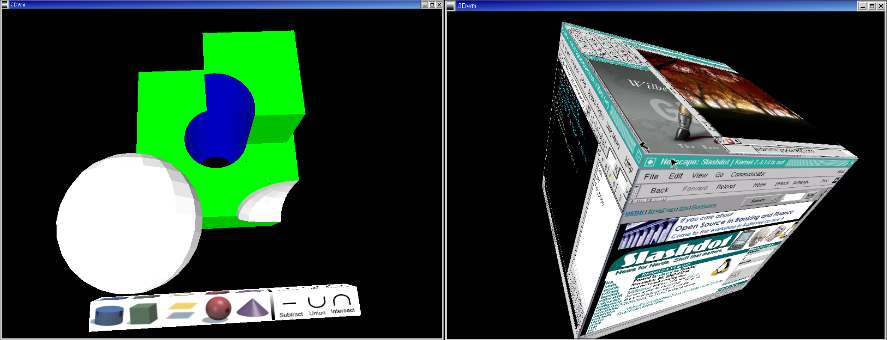
\includegraphics[width=1.0\textwidth]{images/3dwm.png}
\caption{The Three Dimensional Workspace Manager \protect\cite{3dwm}. On the left is a constructive solid geometry modeller, demonstrating the support for 3D applications. On the left we see it texturing multiple X11 desktops (over VNC) onto a 3D cube.}
\end{figure}

Unlike the system described here, but much like early uses of X, their display server draws user interface primitives on the behalf of the client and does not allow the clients to directly control the way the primitives are drawn. This is done because (like early X) network transparency was one of their core design goals, and transmission of pixel buffers from real-time graphics applications to the display server requires much greater bandwidth and much lower latency than most networks are able to provide. The system described in this thesis avoids this (by sacrificing network transparency) because although it gives the system a unified look and feel, it requires that applications perform many transactions with the display server in order to accomplish basic user interface tasks and limits the behaviour and appearance of application user interfaces to functionality supported by the display server. These are the same factors which led to the abandonment of the widespread use of X11's primitive drawing capability and the loss of its pure network transparency (through the use of direct rendering extensions to X) and are two of the major factors motivating the development of Wayland as a replacement for X. 

3DWM does support multiple application contexts in a single 3D space, and allows applications to request volumes for their personal use, which is very similar to the concept of 3D windows presented in this thesis (and is compared to the concept of windows by the authors). However, unlike traditional windows, and unlike the 3D windows presented in this thesis, client applications do not have full control of what is drawn inside of their windowing context. Instead, clients are only able to request that the display server draw primitives inside of their volume, and if the primitives the display server provides do not meet the needs of the application then the developers have no choice but to modify the display server.

Another shortcoming of 3DWM is the lack of native support for 2D windows inside the 3D application space. While the need to support 2D applications is not ignored completely, it is viewed as 'legacy' support during a 'transitionary phase' to completely 3D interfaces and as such 2D applications are not treated as first class clients of the display server. Instead, they implement a custom VNC client which writes a remote desktop into a texture which the display server then applies to a surface in the 3D space. While this does indeed provide simultaneous support for 2D applications running on many platforms, it does not allow individual 2D and 3D applications to be mixed and used together in the same 3D space. 

\chapter{Implementation}
\label{sec:implementation}
This section describes the implementation of the design discussed in Section~\ref{sec:design} built on top of the Wayland display server protocol. This implementation, called `Motorcar', is free and open source and available on GitHub \cite{motorcar-github}. It is intended both to demonstrate concretely that such a design is practical to implement, as well as to serve as a functional 3D windowing system and provide a modular core of that can form the basis of further research into the concept of 3D windowing systems.

\section{Wayland Protocol Extensions}

The design outlined in Section~\ref{sec:design} requires several pieces of functionality not provided by the core Wayland protocol (like synchronization of the view and projection matrices between the compositor and the clients) and functionality that is not supported by the subsystems on which Wayland in built (like the ability for the compositor to access client depth buffers), so an implementation on top of Wayland requires several extensions to the Wayland protocol to provide 3D windowing services to clients (see Section~\ref{sec:wayland-protocol} for a brief introduction to the Wayland protocol).

These protocol extensions form the basis of the 3D windowing mechanism, and are not exclusive to the compositor framework or client applications presented here. Any Wayland compositor or client could hypothetically support these extensions, allowing the basic 3D windowing mechanism to be extended to a variety of applications and integrated with client applications and tool kits as needed. The extensions are designed to be simple and flexible, so that any shortcomings of the compositor and client frameworks presented here do no limit the adoption of the 3D windowing techniques which they implement.

\subsection{Interfaces}

The protocol extensions used by Motorcar define several interfaces which the compositor uses to advertise and provide 3D windowing services to clients. Each of these interfaces is designed to provide one or more of the elements of the architecture outlined in Section~\ref{sec:design}, which is designed to require minimal extensions of existing windowing systems, so the interfaces outlined here are relatively simple.

\subsubsection{Motorcar Shell}

The first interface, `motorcar{\_}shell' represents a compositor shell that supports 3D windowing of the style discussed in this thesis, and  it has a single request, `get{\_}motorcar{\_}surface', which takes an existing Wayland surface (wl{\_}surface) as an argument and returns a new Motorcar surface which is associated with the argument Wayland surface within the compositor.  The compositor creates a single instance of this interface at startup, and clients can then use this instance to create a Motorcar surface object from the Wayland surfaces which they have already created.

\subsubsection{Motorcar Surface}

The interface `motorcar{\_}surface' represents a 3D window of the kind discussed in this thesis. It allows the client to request the type of 3D window desired (for example a cuboid or portal window) and declares events which allow the compositor to inform the client of the 3D window's bounds and transform in space and to deliver 3D input events to the client. Because the instantiation of this interface takes a Wayland surface as an argument, it allows the compositor to identify which surfaces are being used as Motorcar surfaces and composite them appropriately. When a Motorcar surface is created the compositor calculates the buffer size needed to hold the images (and depth buffers) for all of the viewpoints and resizes the surface to these dimensions.

\subsubsection{Motorcar Viewpoint}
\label{sec:viewpoint}

Perhaps the most important of the interfaces defined in the Motorcar extensions, `motorcar{\_}viewpoint' represents a virtual camera in the 3D interface space managed by the compositor (usually corresponding to one of the user's eyes), and provides the mechanisms needed to ensure that the client's 3D content is projected in a manner which allows it to be properly composited with 3D content from other clients and the compositor. This interface has no requests, only events which allow the compositor to inform clients of the parameters for the viewpoint which it represents.

The compositor creates a global instance of this interface for each viewpoint from which it is drawing the scene, allowing the client to produce correct output for each of these viewpoints. The protocol imposes no limit on the number of viewpoints or how the images produced by clients for each viewpoint are laid out within the surface, and allows viewpoints to be added or removed at runtime if necessary, leaving these things up to the compositor implementation. The example compositor presented here supports only a single user and a single stereoscopic display, and does not support hotplugging displays, so it will never instantiate any viewpoints other than the two it creates at startup (one for each of the user's eyes), but this limitation is not reflected in the protocol itself. The Motorcar viewpoint interface defines three events. 

The first two events, `view{\_}matrix' and `projection{\_}matrix', allow the compositor to update the view and projection matrices used by the client, and are sent once when the client connects, and again every time one of the matrices changes. These matrices are updated by separate events because while the view matrix changes every time the user's head moves, the projection matrix changes only when the user's head move relative to the display surface, which never happens when using an HMD (since it is strapped to their head) so the projection matrices for HMD viewpoints never changes at runtime. Some other types of immersive displays, like CAVEs, would require that the projection matrix change every time the users head moves, and while this is compatible with the protocol, it is not supported by the example compositor presented here.

The third event, called `view{\_}port', informs the client of where in the surface buffer to draw the output for the viewpoint generating the event. This allows clients to send the output of multiple viewpoints to the compositor using a single surface, which eliminates the need to synchronize updating multiple surfaces. The view port events actually defines two viewports for each viewpoint, one for the color image and one for the depth buffer, which is needed to correctly composite the 3D content from different clients (see Section~\ref{sec:depth-compositing} for details). It may seem unusual that the color and depth buffers be given different view ports in the same image, since they represent information about the same set of pixels, but this is tragically unavoidable for reasons that are somewhat complicated.

\paragraph{EGL and the Depth View Port}
\label{sec:depth-viewport}

The use of a second view port in the color buffer to transfer the contents of the depth buffer from the clients to the compositor is a significant workaround resulting from the inability of Wayland EGL to make client depth buffers accessible to the compositor. Wayland EGL allows clients to create OpenGL contexts in which the color buffer attached to the default framebuffer can be used by the compositor as a texture without ever needing to copy the memory which backs the color buffer, making it very desirable for clients which are drawing their window on the GPU (as any 3D application would certainly be doing). However, Wayland EGL does not give the compositor the same kind of access to the depth buffer attached to the default framebuffer in the client's context, which presents a significant hurdle. 
	
This is overcome by doubling the size of the color buffer attached to the client's default framebuffer, drawing into a framebuffer object whose color and depth buffers are backed by textures, and then texturing both the color buffer and the depth buffer from the framebuffer object into the color buffer attached to the default framebuffer. The compositor can then extract the original depth and color buffers from the client color buffer and write them back into the depth and color buffers of a new framebuffer, which it can then composite with the 3D scene based on the contents of the depth buffer. This introduces a significant amount of rendering overhead and is the only part of this design that cannot currently be implemented cleanly on top of Wayland. Solving this problem efficiently, by giving the compositor direct access to the depth buffer attached to the client's default framebuffer, is probably possible but would likely require modification of the implementation of Wayland EGL within Mesa. This is considered by the author to be the single most pressing area of future work on this system.

\begin{figure}[ht!]
\centering
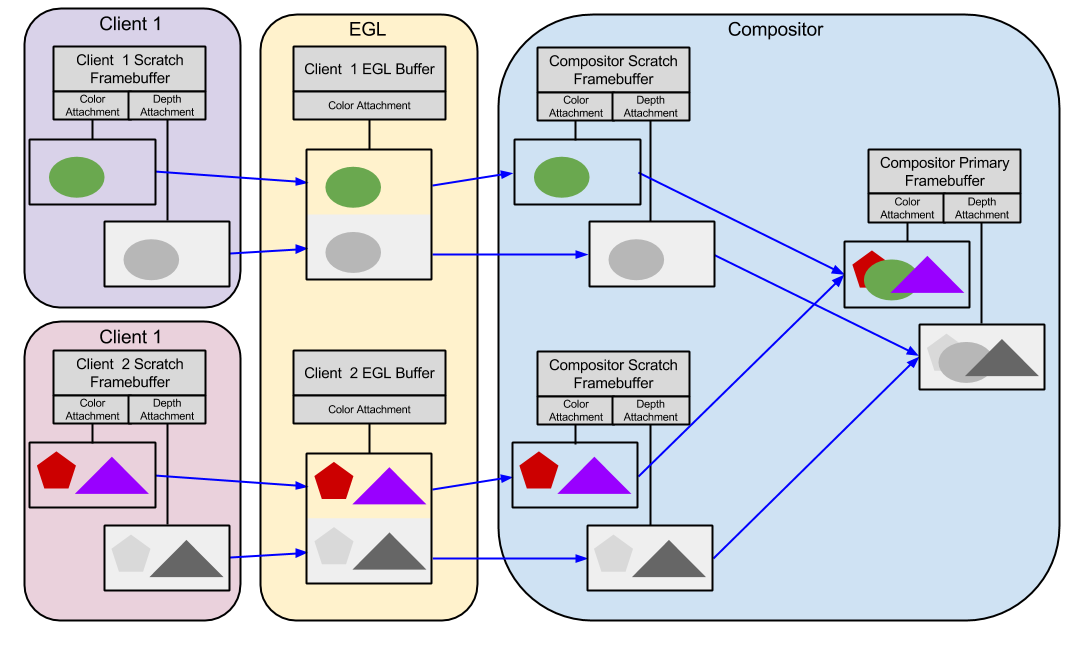
\includegraphics[width=1.0\textwidth]{images/depth-buffer-operation.png}
\caption{A high level conceptual illustration of the depth compositing process. Clients draw their depth and color images into the same, double-height color buffer, which the compositor then draws back into normal sized depth and color buffers, and then composites with other 3D clients using the traditional depth test. Lighter color in the depth images indicates that those pixels are further away.}
\end{figure}

The process of encoding the depth buffer contents in the color buffer is further complicated by the differences between the format of the depth buffer and color buffer. The example compositor uses a color format that allocates eight bits for for each of four color channels (red, green, blue, and alpha, which is used here for transparency) and a 16 bit integer depth format. In order to transfer the depth information without loss of precision the system presented here samples the depth buffer on the client side as a 32 bit float, then uses a technique taken from \cite{pack-float-rgba} to pack this float into a four-vector which is then written into the color buffer and unpacked back into the 32 bit float on the compositor side (using the reverse technique from \cite{pack-float-rgba}) and written back into the depth buffer. 

\subsection{Current Protocol Limitations}
In its current state the Motorcar protocol extensions has very basic support for 3D input events. The only implemented input events are essentially the 3D equivalent of mouse events, such as button pressed attached to a six degree of freedom (6DOF) transform, or changes in this 6DOF transform. These kinds of events form a good extension of mouse events to 3D, and map well onto the input device used in this implementation (the Razer Hydra 6DOF handset), but they certainly do not encompass all possible 3D input. Other broad classes of input events include skeleton tracking and gesture events, and these types of events could certainly be delivered over additional Wayland protocol extensions. However, an abstraction layer for these types of events would require the development and integration of substantial systems which are well outside the scope of this thesis, so they are excluded from this version of the Motorcar protocol extensions.

\section{Client Operation}

This section describes the operation of 3D clients using the Motorcar protocol extensions, and most of this is firmly grounded in the way that the sample 3D clients provided by Motorocar operate. The operation of 2D clients is not discussed in detail here because it is literally identical to standard Wayland client operation, which is a key feature of this system because it allows unmodified 2D clients to window into the 3D interface space without even being aware of its three dimensional nature. The example Motorcar client code is derived from the weston-simple-egl client distributed with Weston (the Wayland reference compositor), but adapted from C to C++ and repackaged as an interface which can be implemented by individual clients with minimal effort.

When the client connects to the compositor it receives creation events for all of the global objects instantiated by the compositor, including the Motorcar shell and all of the Motorcar viewpoints. The client can use the Motorcar shell to create a Motorcar surface from any Wayland surfaces it create, which tells the compositor to handle that surface as a Motorcar surface (since these are composited differently than normal surfaces) and allows the compositor to send 3D input events to that client, which the client can listen for if it chooses. 

The client binds each viewpoint and creates a data structure to represent it internally, which it then attaches to the event listener for that viewpoint. The compositor responds to the binding process by sending the client the current state of the viewpoint (its view and projection matrices and its view port) to the client, which the client then stores in the data structure associated with that viewpoint.

Every time the client gets the frame callback indicating that it should draw a new frame, it iterates over all of the viewpoints and draws it's scene however it likes with the view and projection matrices from that view point into the viewpoint's color view port, then copies the depth buffer for that viewpoint into the viewpoint's depth view port. Once this has been done for each of the viewpoints the client calls eglSwapBuffers, which swaps the surfaces front and back buffers and informs the compositor that surface is ready to be updated.

\section{Compositor Operation}

This section describes the operation of the Motorcar compositor implemented for this thesis. There are other ways that a Motorcar protocol compliant compositor could function, but enumerating all of these designs is an intractably large task and likely would not be useful anyway, so instead this section focuses on the concrete aspects of the design that was implemented and is known to work. The operation of the compositor is complex, and an exhaustive discussion of this software that implements it would be obscenely long, so the discussion here is limited to the components of the compositor which are relevant to the mechanism by which is provides 3D windowing services to clients. Users seeking a more comprehensive understanding of the structure of this software are directed to the documentation in the GitHub repository \cite{motorcar-github}.

\subsection{The Motorcar Compositor Framework}

This thesis presents a modular C++ framework for Motorcar compositors designed to be extremely flexible in the way that 3D windowing services are provided to clients. The main function of a compositor built with this framework essentially just initializes components which implement interfaces defined in the framework and attaches them to one another over these interfaces. This allows components which do not meet the needs of a particular compositor to be replaced by ones that do without needing to rebuild the compositor from scratch, and it allows new components to be defined and attached in natural ways. Examples of modules which would likely be replaced are device specific classes (which implement device interfaces for things like 3D pointing devices or head mounted displays on top of device specific API's) and the window manager (which controls how input events are directed to clients and how surfaces are laid out in 3D when they are mapped).

\subsubsection{The QtWayland Motorcar Compositor}

The Motorcar compositor implemented for this thesis uses several core components built on top of the QtWayland Compositor API. QtWayland is a module in the Qt toolkit which provides a Wayland backend for graphical Qt applications, as well as providing a simple framework for building Wayland compositors on top of Qt. All of the QtWayland dependent functionality in this compositor is isolated within a small set of classes which hide the QtWayland functionality behind interfaces defined in the Motorcar framework, which could hypothetically allow it to be separated and allow Motorcar compositors to be built without a Qt dependency, though this is not necessarily desirable.  

QtWayland abstracts almost all of the interaction with the Wayland protocol itself (with the exception of interactions with the Motorcar protocol extensions) behind a set of C++ classes which form the QtWayland Compositor interface, and most of these classes interact with the Motorcar compositor framework through thin wrapper classes which exist primarily to isolate the Qt dependency. It handles almost all of the behaviour needed to correctly interact with 2D clients, allowing the Motorcar compositor framework to focus on embedding the 2D clients' surfaces in the 3D space and correctly sending these surfaces input events in their local coordinate system. Additionally, Qt provides a platform independent OpenGL context, which allows QtWayland compositors to run within other Wayland Compositors, within an X environment, or even directly on top of the user interface hardware abstractions in the Linux kernel.

\subsubsection{The Compositor Scene Graph}



The compositor maintains an internal scene graph which contains all spatial elements in the 3D interface space. This includes surfaces (for both 2D and 3D windows), viewpoints, displays, input devices, models of the user skeleton, and any graphical interface elements drawn by the compositor (for example window decorations or docks). All scene graph classes inherit from a root class called SceneGraphNode, which provides spatial relationship primitives as well as defining a doubly linked tree structure between nodes (which forms the actual graph of the scene) and provides mechanisms for traversing this tree. 

All scene graph nodes have a single parent and a list of children, and these are made accessible so that other parts of the compositor can manipulate the scene graph as they see fit, and these two members form the core of the functionality that the SceneGraphNode class provides. The scene graph is rooted in an instance of a special scene graph class called Scene (which is unique in being allowed to have a null parent), and this forms the primary interface between scene graph classes (which can always access the scene root by traversing up the scene graph) and classes like the window manager, motorcar shell, and display server modules (which typically are constructed with a pointer to the scene on which they operate).

\begin{figure}[ht!]
\centering
\includegraphics[width=1.0\textwidth]{images/scene-graph-classes.png}
\caption{The inheritance graph for the classes composing the scene graph. Note the division between virtual nodes (which can be children of any other node) and physical nodes (which can only be children of other physical nodes) to reflect the impossibility of a physical object being attached to a virtual one.}
\label{fig:scenegraph-classes}
\end{figure}

\paragraph{Traversing the Scene Graph}

The scene graph is designed to be traversed several times per frame, and the SceneGraphNode class provides virtual methods which allow implementing classes respond to each of these traversals appropriately without needing to implement the traversal logic themselves. The first traversal, invoked immediately prior to sending the current viewpoints to the clients and requesting new data from them, is intended to allow implementing classes to do per-frame work prior to rendering (for example animation updates or event generation by devices) and is handled by overriding SceneGraphNode::handleFrameBegin(). The second traversal, invoked once per display per frame, is intended to allow implementing classes to render their content to the display and is what drives surface classes to perform the compositing operations discusses in Section~\ref{sec:3d-compositing}. This traversal can be handled directly by overriding SceneGraphNode::handleFrameDraw(), but most classes that respond to this traversal should inherit Drawable and override Drawable::draw() instead. The third and final traversal, invoked every frame after drawing is completed and handled by overriding SceneGraphNode::handleFrameEnd(), in intended to allow any implementing classes to clean up any resources which were created during the first traversal that will not be needed in the next frame.

\subsection{Frame Timing and Latency}

This design requires that the compositor send new view matrices to its 3D clients every frame, wait for them to draw new images, and then composite these images and send them to the display before the next frame starts, so getting the timing correct is a little bit tricky and there are several possible approaches with merit. 

The approach taken in this implementation is to draw the scene graph (the handleFrameDraw traversal) with the current data at the beginning of the frame, clean up the frame (the handleFrameEnd traversal), update the scene graph state (the handleFrameBegin traversal), then send the new matrices to the clients followed by the frame callbacks that tell them to draw a new frame, then wait until the next vSync event (indicating the display is done drawing) to swap the compositor buffers and restart the process. This approach favours using old client output over dropping frames in the compositor because it gives clients only the time remaining in the frame after compositing completes to update their content before the compositor simply uses the output it already has in memory. This ensures that no single client can reduce the compositor frame rate, but it also means that 3D clients can get out of sync with the compositor, which would break the illusion of a unified 3D interface space (because out-of-sync clients would be drawn from a viewpoint that has since changed). Additionally, this means that the time it takes a movement of the user's head to affect the image drawn appropriately (referred to as `motion-to-photon latency') would include an entire extra frame's worth of time, which is undesirable in certain applications.

An alternative approach would be to update the scene graph, send the new matrices and frame callbacks to the 3D clients, wait until all of the 3D clients have finished drawing, and only then draw the scene and clean up. This approach would minimize the motion-to-photon latency but, because it requires that the compositor wait for the clients to finish drawing, it could allow a single slow client to cause the compositor to drop frames. This approach may be more suitable for applications like immersive virtual reality video games, where only a single latency-sensitive application needs compositing, and it is probably not the most general purpose solution. As discussed in Section~\ref{sec:vr-mode}, this timing mode could potentially be toggled from the client based on its application profile, though such functionality is not yet implemented in the system presented here.

\subsection{Three Dimensional Compositing}
\label{sec:3d-compositing}

The core functionality of a Motorcar compositor is its ability to combine interfaces from 2D and 3D applications in a unified 3D interface space. The compositing portion of this requires that the compositor be able to draw 2D windows on planes embedded in the 3D space and be able to composite the output from 3D applications with these planes as well as with the output of other 3D applications. The first requirement is fairly straightforward (especially with the use of QtWayland), essentially boiling down to projecting and texturing quads with OpenGL, so we do not bother to discuss it in detail here. The second requirement is met with a fairly complex mechanism that forms one of the core contributions of this thesis, and this mechanism is the focus of the rest of this section.

When clients create a Motorcar surface, the scene graph node representing the surface (of class WaylandSurfaceNode) is replaced by a new node with an inheriting type (class DepthCompositedSurfaceNode)  that defines the correct compositing behaviour for Motorcar surfaces. The DepthCompositedSurfaceNode class performs the compositing operations needed to make the contents of its surface appear three dimensional to the user.

\subsubsection{Clipping and Depth Compositing}
\label{sec:clipping-impl}

The clipping process varies slightly depending on the type of window being clipped, but for the most part the process is identical. The term `near clipping surface' is used here to describe the surface which the everything in the window must be in front of, the term `far clipping surface' is used to describe the surface which everything in the window must be drawn in front of, and `full clipping surface' is used to describe the union of these two. For a cuboid window the near clipping surface is the three faces of the cuboid facing toward the viewpoint (the first three faces where the dot product of the face normal and the view vector is less than or equal to zero) and the far clipping surface is the other three faces of the cuboid. For portal type windows the near clipping surface is the window opening and the far clipping surface doesn't exist. The depth compositing and clipping process uses a scratch framebuffer with the same dimensions as the compositor buffer and the process described here operates once per viewpoint.

This scratch framebuffer is first cleared (zeroing the red, green, blue, and alpha values), and the full clipping surface of of the window is written into the stencil buffer (such that only pixels within the projection of the clipping surface can be drawn to) with the color and depth buffers disabled. This prevents the client from drawing any fragments which can not possibly be valid because they are outside the projection of its window bounds, and substantially reduces the overhead of copying pixels because pixels disabled by the stencil buffer will simply be ignored. The next step is to draw the client buffer into the color and depth buffers of the scratch framebuffer using the late depth test (the depth image is extracted from the client color buffer, due to the problem described in Section~\ref{sec:depth-viewport}). This draws only those pixels which are closer than the far clipping surface, since those which are further away will fail the depth test. This draw is also where the stencil buffer drops all fragments outside the projection of the window. Next, the near clipping surface is drawn into the color and depth buffer with a completely zero color (including alpha), blending disabled, and the depth test reversed (so that fragments with greater depth pass the depth test). This replaces any fragments from the client image which are closer than the near clipping surface with the scratch framebuffer's clear color, effectively eliminating them. Finally, the contents of the scratch framebuffer (both depth and color) are drawn into the compositor framebuffer using the late depth test and a special fragment shader which drops fragments whose alpha values are zero, which prevents the depth of the clipping surfaces from polluting the compositor depth buffer. 

This process ensures both that any fragments in the client buffer which lie outside the window bounds are discarded and that any fragments inside the window bounds are composited properly.


\section{Test Hardware Configuration}

This compositor was developed using an Oculus Rift DK1 virtual reality headset and a Sixense Razer Hydra six degree of freedom magnetic tracking handset system. The Rift provides only head orientation tracking, which does not allow proper motion parallax to be simulated (see Section~\ref{sec:motion-parallax-and-stereopsis} for details. Fortunately, the Hydra system comes with two handsets, which allows one to be used to track the head's position (by attaching it to the back of the Rift headset), while the other is used as an input device. This setup can be seen in Figure~\ref{fig:hardware-setup}.

\begin{figure}[ht!]
\centering
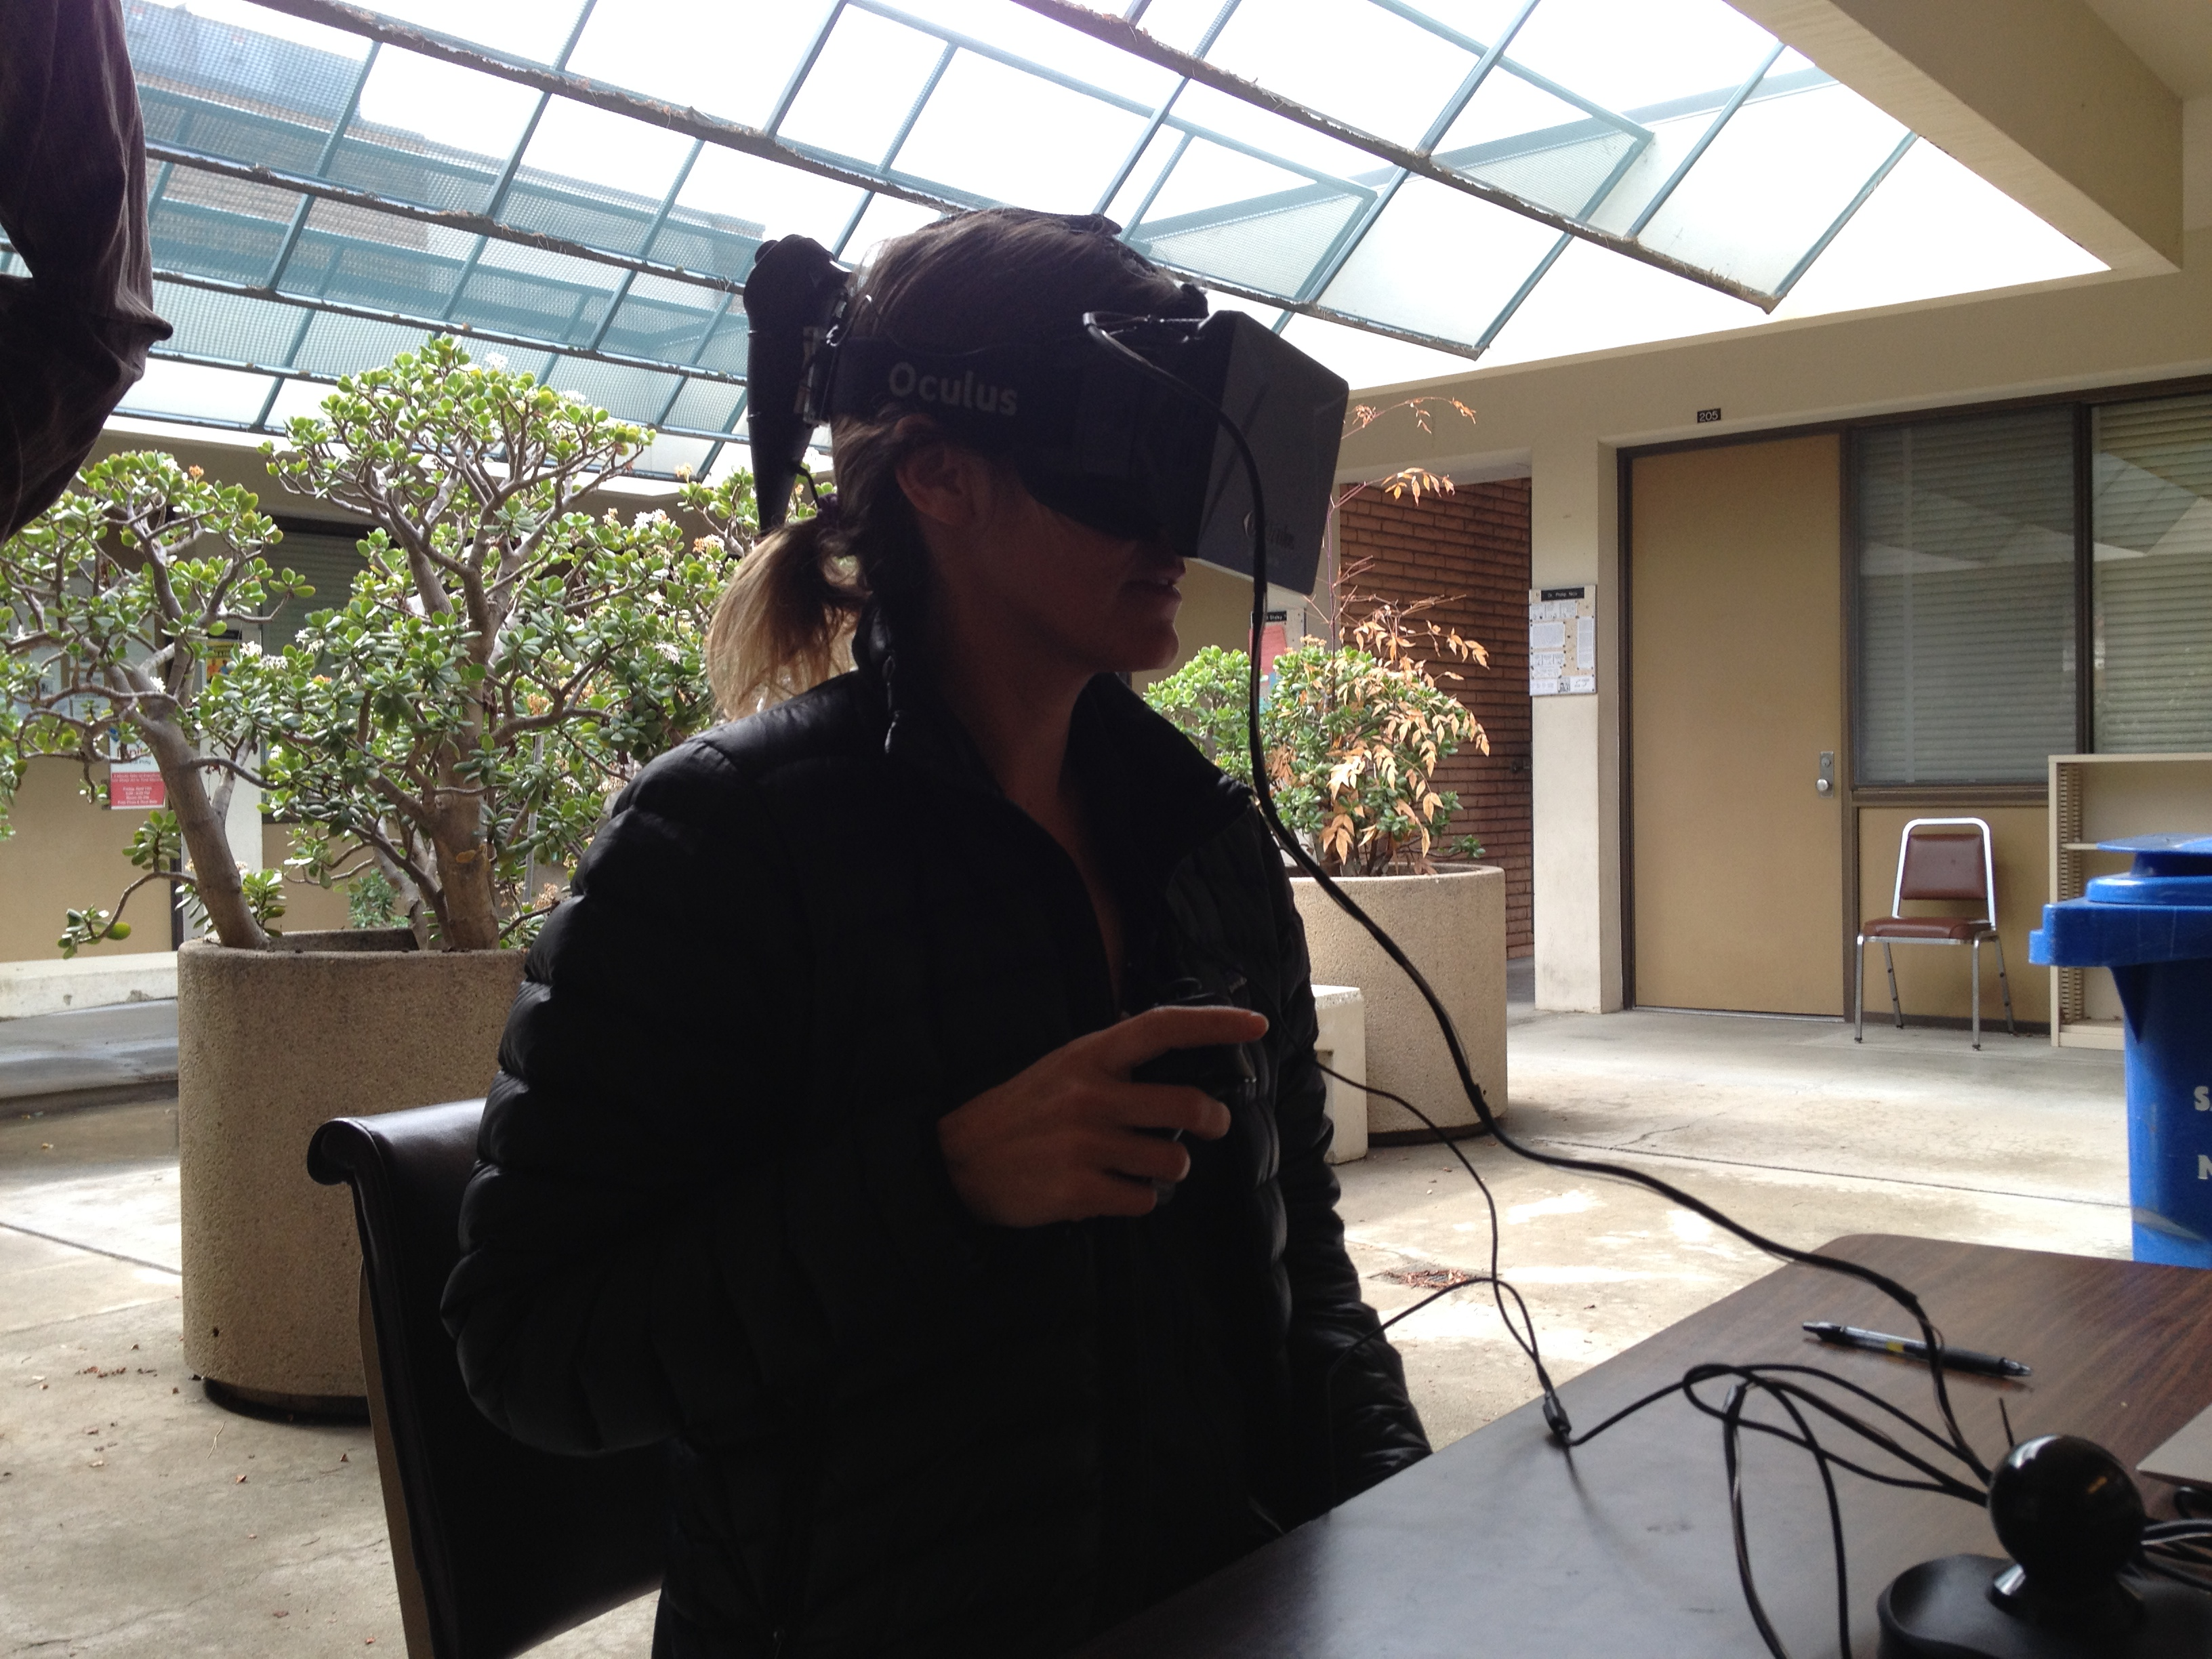
\includegraphics[width=1.0\textwidth]{images/hardware-setup.jpg}
\caption{A test subject wearing the hardware system on which this implementation was developed. Notice that one Hydra handset is held in her right hand and being used for 3D input, while the other is attached to the Rift headset and used for traking the position of the head.}
\label{fig:hardware-setup}
\end{figure}

The Oculus Rift requires a image space barrel distortion of the rendered stereo image to correct for a pincushion distortion introduced by the optics in the headset. This is performed as a final step immediately before the compositor sends the final image to the display. Clients need not even be aware of this step, which is yet another advantage of using the windowing approach described here.












\chapter{Results}

\section{Experimental Setup}

To understand the differences between the juicy and juice-less versions of POOP-SNOOP and evaluate my prototype, two experiments were executed. 88 Cal Poly undergraduate students and professors anonymously reviewed only the ``juicy" version of the game while 45 students and professors anonymously reviewed only the ``juice-less" version. In a separate experiment, a separate group of twelve Cal Poly students reviewed both ``juicy" and ``juice-less" versions of the game side-by-side while accompanied by a proctor.

The ``juicy" and ``juice-less" prototypes contained exactly the same text, shapes, slides, and order. The intension was to isolate juiciness, and the specific differences were identified in the Implementation Section. In the prototype, the users first completed the tutorial section which led directly into a introductory level for participants to utilize their new skills. When the puzzle had been arranged in the optimal solution, they were told that the best solution had been solved, though they were still allowed to continue playing that puzzle.

\subsection{A/B Testing}

To gather subjects, an opportunity to participants was presented to four classrooms of 20-30 students. More participants were only given the option to participate via email. All participants were given an introduction verbally or via email. The introduction briefly outlined the purpose of citizen science games, and basic instructions to complete. The essential instrutions were embedded in the game itself. 

Within the game, subjects were asked to fill out a anonymous feedback form after the tutorial section and then another anonymous feedback form after playing an introductory level. The anonymous feedback forms used can be found in the appendix.

\subsection{Focus Group Testing}

Ten of the focus group members study a design-related subject, but none of them were involved in a computer science related field. Zero of these participants had played a citizen science game before.

Each focus group member played both versions of the prototype while being observed. They were allowed to ask questions about clarifications and encouraged to speak about their emotional response to the prototype while they played. Half of the subjects played the juiceless version first, and the second half played the juicy version first. Before the subjects were given a prototype, they were told about the nature of citizen science games some details about the origins of the data used in POOP-SNOOP. Zero participants filled out the surveys, each only provided verbal feedback.

\section{Evaluation}

The most significant observations from the A/B testing are:

\begin{enumerate}

\item Users completing the ``juicy" tutorial tended to have higher confidence about solving POOP-SNOOP puzzles.

\item Users completing the ``juicy" tutorial indicated more interest continuing after the tutorial to solve POOP-SNOOP puzzles.

\item Users playing the ``juicy" introductory level found their puzzle less difficult.

\item Users playing the ``juicy" introductory level indicated that the tutorial was more helpful than ``juiceless" players.

\item Users playing the ``juicy" level indicated more enjoyment of POOP-SNOOP than ``juiceless" players. 

\item Frustration with fundamental game mechanics and tutorial unclarity was voiced by more ``juiceless" players than ``juicy" players.

\item More ``juicy" prototype players specifically mentioned encouraging graphics.

\end{enumerate}

From the focus group study, observations concluded: 

\begin{enumerate}

\item The chevrons were helpful in indicating the primary mechanic in both ``juicy" and ``juiceless" prototypes.

\item The ideal POOP-SNOOP would be comprised of features from both the ``juicy" and ``juiceless" prototypes.

\item There was excessive feedback when making changes to the solution to the point that it interfered with solving the puzzle.

\item The incremental ``juicy" feedback regarding different sized solutions was not effective.

\end{enumerate}

\subsection{A/B Testing}

The two surveys given during each A/B testing session, the first after the tutorial and the second after the introductory level. The appendix lists the two surveys distributed. Table \ref{table:tutorialsurvey} is the summary of these qualitative results from the post-tutorial survey. Table \ref{table:gamesurvey} is the summary of quantitative results from the introductory level of POOP-SNOOP. Participants of the ``juiceless" experiment completed 58 post-tutorial surveys and 43 final surveys. Participants of the ``juicy" experiment completed 54 post-tutorial surveys and 66 final surveys. It is not clear why there were not an equal number of surveys completed for each version of POOP-SNOOP, but without any insight into the reasons for the discrepancy none of the results were discarded.


\begin{table}
\begin{center}

\begin{tabular}{|>{\centering}p{3cm}|c|c|c||c|}
\hline 
Question&  Mean Juicy&  Mean Juiceless&  Difference&  p-value
\tabularnewline
\hline 
How confident do you feel about solving a POOP-SNOOP puzzle?&  3.0&  2.3&  1.3&  0.003
\tabularnewline
\hline 
How interested are you in solving a POOP-SNOOP puzzle?&  3.3&  2.5&  0.8&  3.1E-5 
\tabularnewline
\hline 
\end{tabular}

\caption{Comparison of the difference in confidence and interest between players of the ``juicy" and ``juiceless" prototypes}
\label{table:tutorialsurvey}
\end{center}
\end{table}

All quantitatively measured results from the surveys were statistically significant (p-value $<$ 0.05), the results are listed in Table \ref{table:tutorialsurvey} and Table \ref{table:gamesurvey} and summarized in the beginning of this chapter.

In the ``juiceless" version, 45 of 58 responses cited confusion about game mechanics, purpose, or goal, where only 17 of 54 ``juicy" participants agreed. There may be a connection between making interesting tutorial levels that increases players attention to learning the game or reading text. Players found the ``juicy" version more enjoyable, and 5 of 66 responses specifically mentioned that the ``juicier" graphics were encouraging and helpful, though they had not seen the ``juiceless" version.

Surprisingly, 6 of 43 ``juiceless" players specifically mentioned ``visually clean", ``great interface", ``clean presentation", or praised the visual design. Another astonishing comment from the ``juiceless" survey suggested, ``You need to make the game juicy" and included a link to the talk by Martin Jonasson \cite{juiceitorloseit} that inspired this project. Two other comments in the non-juicy version also mentioned adding color and doing more user testing. These comments were not ordinary, most comments did not mention anything about the design or the ``juicy" design of POOP-SNOOP.

\begin{table}
\begin{center}

\begin{tabular}{|>{\centering}p{3cm}|c|c|c||c|}
\hline 
Question&  Mean Juicy&  Mean Juiceless&  Difference&  p-value
\tabularnewline
\hline 
Did you enjoy POOP-SNOOP?&  3.0&  2.4&  0.6&  0.00147
\tabularnewline
\hline 
Was the puzzle difficult?&  2.4&  3.5&  1.1&  2.8E-7
\tabularnewline
\hline 
Was the tutorial clear and helpful?&  2.4&  1.7&  0.7& 0.00045
\tabularnewline
\hline 
\end{tabular}

\caption{Comparison of the difference in enjoyment, perceived difficulty, and understanding between players of the ``juicy" and ``juiceless" prototypes}
\label{table:gamesurvey}
\end{center}
\end{table}

\subsection{Focus Group Testing}

In every focus group interview, each subject came to the conclusion that the ideal puzzle would contain features of both the juicy and non-juicy versions (overview result 2). When asked to make a choice about which version they would prefer to play another puzzle with, four subjects responded ``juicy" and eight responded ``juiceless".

Subjects tended to prefer the non-juicy version, even if they had been given the juicy version first. Users cited the distracting ``juicy" feedback interfered with their ability to solve puzzles. Users preferred the quicker response of the ``juiceless" version.

Players quickly became annoyed by the overwhelming response of the system for every time they moved the puzzle orientation (overview point 3). The first time the rewarding animations happened, subjects were excited, but it became repetitive quickly. 

The scoring animations were slightly more intense if the score was larger, but no subjects noticed the different between any of the animations (overview point 4). The range of possible solutions was between 2 and 4, restricting the number of animations. There was not enough variation between the response to solutions and the response was too intense for every solution. Participants suggested that the background animation should only reward them the first time they create large solution.

The scoring animations caused player confusion when removing grid blocks that were not part of the solution. Four participants explicitly stated that they thought the puzzle was restarting or changing when the blocks dissapeared and reappared. The emphasis of the solution was inadequate; no players mentioned specifically preferring this behavior.

The chevrons for the diagonal squares were effective in both the juicy and juiceless versions (overview point 1). Early in our prototype process, the grid was simply an array of plain squares with no special markings. There was consistantly a problem with people understanding the core mechanic of POOP-SNOOP: the diagonal drag. Because the grid looked square, subjects always attempted to drag row-column pairs in any direction and simply allowing motion only in the diagonal direction never caught on. Eventually, the idea for chevrons on the diagonal was implemented and to my surprise ten out of twelve focus group participants naturally grabbed the squares along the diagonal and dragged them in the correct direction. The two that didn't understand the dragging motion immediately did not interact with the tutorial phases until they were forced too and seemed to skip the instruction about movement.

The lack of colors in the ``juiceless" often caused confusion in the tutorial because the grays were indiscernible. More subjects interacted with the ``juicy" tutorial when the puzzle first appeared on screen. The three observed participants who played with POOP-SNOOP before the introductory level started had the most success with understanding.

\chapter{Discussion}

\section{The Language of Juiciness}

One of the most important asepcts of designing an experiment around POOP-SNOOP is measuring ``juiciness". The language of ``juicy" design doesn't coincide with players vocabulary. The question, ``is this game juicy?" might invoke some good guesses, but it is not perfect. Without knowledge of the difference, players would likely not discern between the experience of the game and the game itself. But again, is the game what should be measured? If games specifically create experiences, is measuring the experience the same as measuring the game? 

The concept of ``juiciness" is defined by the experience created while playing the game. Atanasov \cite{atanasov} states that a juicy experience could be defined as plentiful ``positive emotional feedback", but those words are charged with implications and may skew the results if players were asked to describe any ``positive emotional feedback" they experienced during play.

While players were interviewed, they found it difficult to describe their emotional state. Instead, they verbalized their feelings about of the game. Interviewees pointed out specific aspects they liked whether the smoothness of the interface, the way the chevrons highlighted and bounced, or the flourishes of the background animations. While these emotions are aligned to a positive or negative emotion, the overall emotional response is more difficult to analyze. At which point do certain negatives outweight positives?

Putting POOP-SNOOP in the hemisphere of citizen science reveals a convenient definition of ``positive emotional feedback". In citizen science games, players should feel motivated and encouraged to continue solving puzzles. Asking a player if they would continue playing POOP-SNOOP is not the same measurement as real citizens playing POOP-SNOOP. Because of the nature of my prototype, users were not given the ability to pursue more puzzles. We have sufficiently answered the question that with regards to citizen science games, juiciness can have a substantial impact on player attentiveness.

\section{Juiciness and Game Feel}

Collecting data about playing POOP-SNOOP has demonstrated that ``juicy" is only part of a larger feeling of gamefulness. Like game feel suggests, mechanics play an important role in the quality of a game. Players are susceptible to juiciness' influence while learning about the mechanics of a game, as those who played the ``juicy" tutorial have demonstrated, but there were still plenty of players who mentioned confusion after completing the game. Did their confusion inhibit their ability to answer the survey questions correctly? Would they have been able to answer the survey if they were confused? In this situtation, those results were utilized because there was a tendency for players of the ``juicy" version to be confused less. The experiment shows those those who played the ``juicy" version potentially learned the game better. The goal of ``juiciness" is only to reinforce the mechanics and physicicalilty of the game, but if players cannot understand those concepts, measuring their sense of experiencing ``juiciness" could potentially be misleading.

\subsection{Juiciness and POOP-SNOOP}

Several aspects of playability in POOP-SNOOP potentially interfered with players' willingness to reflect on subtleties that were not playable aspects. For instance, when the introductory puzzle interrupted players with exaggerated congratulations, did they take that into account when the measured ``enjoyment"? Enjoyment, interest, and difficulty are not a strictly ``juicy" measurment nor is POOP-SNOOP a perfect example of ``juicy" and ``juiceless" design. Playability is an important fundamental in enjoyment.

Because some users of the ``juiceless" version praised the clean layout, it's worth mentioning that there may have been extra ``juicy" effects in the ``juiceless" version. By definition, the ``juiceless" version should be a version of the game that has very little visual design additions. While the earlier definition only applies to effects, particles, sounds which are all easily grouped, where does overall design fit in this model?

For instance, the design of the grid was as much part of the ``juicy" version as it was in the ``juicless" version. Should the ``juiceless" version have incorporated less visual design, instead of just omitting the particle effects? Did incorporating a simple grid structure break the definition of ``juiciness" provided or is that design fundamental to the mechanics. By measuring different versions of POOP-SNOOP, the intention was to measure the effect of design that was as extraneous as possible, but there are aspects present in both versions that could arguably be ``extraneous". 

Too much polish is distracting because it makes it difficult to wrap your brain around the physical sensation being conveyed \cite{swink2009game}. The little puffs of smoke that come up as Mario slides his feet around are great because they make sense. When every single object has puffs of smoke, how does that reconcile with the experience of physical reality? Though games do not intend to perfectly replicate reality, certain physical sensations make more sense than others. Should ``juicy" affects replicate nature? Or, is the interesting part of ``juicy" effects that they are unexpected? ``Juicy" design fits on this spectrum, but importantly, game designers must take care to associate effects with specific game feedback. Too many extraneous effects are just as confusing as too few.

The harmonization of polish and mechanics support the single impression of physicality \cite{swink2009game}. In a puzzle game, physicality isn't as obvious as an immersive role-playing game. The phsyical metaphor for puzzle games are weak which potentially limits convincing ``juicy" effects. 

\chapter{Future Work}
The thesis presents an architecture for unified 2D and 3D windowing systems, and the implementation, Motorcar, is meant to server both as a proof of concept that this architecture is feasible to implement on top of existing windowing systems and as the basis for an open source implementation of this architecture. As such, the potential for future work based off of this thesis represents a significant portion of the value that it adds to the field. 

\section{Input Events}
The system presented here supports a single type of 3D input event which is strongly analogous to traditional mouse events, only three dimensional. These events map well onto the hardware on which this system was developed (since the Razer Hydra is strongly analogous to the three dimensional equivalent of a traditional mouse), but this class of input events by no means captures all classes of 3D input. Other broad classes of 3D input, some of which are discussed here, could also be handled by the windowing system and delivered to applications abstractly.

\subsection{Skeleton Tracking}
Many consumer grade 3D input devices are designed to track the user's body directly and use this information for input. The APIs which provide the tracking information are typically device specific, though systems which abstract this information from device specific APIs are actively under development. A good example of one such system is Shapansky's Jester \cite{jester}, which not only provides a device agnostic abstraction, but also provides a framework for using multiple skeleton tracking devices to drive a unified skeleton model. 

Integration of such a system into Motorcar would allow it to provide client applications with abstract skeleton input and provide devices an abstract input interface which could be driven off a variety of device specific APIs. This would require that an additional set of protocol extensions be developed to communicate skeleton data to 3D clients, but the author sees no reason why this would not be possible. 

Furthermore, Wayland supports touch input natively, so the skeleton data could be used to generate touch events for 2D windows (whenever the user's fingers intersect the window in 3D space), allowing users to interact directly with 2D applications embedded in the space around them witshout these applications needing to support the extensions which communicate skeleton data directly.

\subsection{Gestures}

Having the windowing system handle skeleton input internally would also allow it to recognize gestures (specific sequences of body movement) and use them to control the windowing system or to deliver them to client applications as input events directly. This would require several new systems to function in the most general sense. 

The first, and perhaps most important, requirement is some way of representing gestures in an abstract and general way so that they can be communicated between systems involved in the gesture input data flow. Such a representation would need to able to represent a broad class of useful gestures (both as a general gesture that could happen and as a specific gesture event that has happened) in a variety of formal language (so gestures could be communicated between systems written in different languages) including the Wayland display server protocol. A set of protocol extensions would need to be created to communicate gestures represented in this form between the compositor and client applications.

The second is a gesture recognizer which can operate on the unified skeleton model to recognize any gesture described in this representation. Because the recognizer can recognize any gesture described in the abstract representation, it could recognize gestures on behalf of many different entities, provided these entities had some channel of requesting that the recognizer listen for their gestures. This means that the windowing system could register gestures for recognition which it could use to control windows, applications could register domain specific gestures for recognition through the windowing systems, and users could configure special gestures which they like to be used for a variety of input purposes.

The third is some kind of training mechanism which would allow users or developers to input a set of movements and then use these movements to generate a description of a gesture in the abstract representation without needing to define the representation explicitly. This could be accomplished by multiple disjoint systems, or it could be integrated into the recognizer, or both.

\section{User Interface Toolkits}

In traditional windowing systems, applications rarely interact directly with the windowing system itself. Rather, interactions with the windowing system is handled by a piece of middleware called a user interface (UI) toolkit. These toolkits abstract higher level interface concepts, like buttons and menues, on top of the windowing system, and applications are built with this higher level components. These toolkits are complex, and the design of such a system is a significant software engineering challenge. 

The development of such a toolkit on top of a 3D windowing system like the one presented here  would allow applications to leverage the capabilities they provide without needing to create their own interface abstractions on top of the windowing systems. There is at least one relatively mature toolkit for building applications with 3D user interfaces, called Vrui \cite{vrui}, but it is designed to run on top of X11. Porting Vrui to run on top of a 3D windowing system may be possible, and would make a large body of 3D user interface research compatible with these systems, but it is unclear whether this is even possible at this time.

\section{EGL Depth Buffer Extensions} 
Motorcar takes a significant performance hit because it needs to copy the client depth buffer in and out of the color buffer in order to make it accessible to the compositor, which adds two rendering passes to the compositing process for 3D client applications. EGL support extensions of the interfaces, and it may be possible to modify the open source EGL implementation in Mesa to natively support making the client depth buffer directly accessible to the compositor internally, eliminating the need for the extra rendering passes. It is not certain that this is possible, but it is likely. This is likely the next thing the author will pursue on this project.

\section{Immersive Vitrual Reality Mode}
\label{sec:vr-mode}
Many of the applications which currently use the hardware that the windowing system presented here is designed to abstract are immersive virtual reality (VR) experiences. These applications are very resource intensive, extremely latency sensitive, and typically are designed to take complete control of the hardware.

The depth compositing process presented here introduces significant rendering overhead, and is only necessary if multiple applications wish to use the 3D user interface hardware simultaneously (which is not the case with VR applications). Therefore it could be useful to allow client applications to enable a special compositing mode which ignores outputs from all other applications (and stops asking them to update), ignores the client depth buffer, and blit the client color buffer directly into the compositor buffer. This would essentially disable the compositing process, minimizing the computational overhead introduced by the compositor (and other clients), and minimizing the latency added by the compositing process.

It may also be useful to allow clients in this mode to request that the compositor update the view and projection matrices at any point in time, allowing VR applications to use the most recent head transform possible. 


\section{Feasibility in Other Windowing Systems}
It is clear that the basic architecture outlined in Section~\ref{sec:design} can be implemented on top of Wayland, since Motorcar demonstrates this by nature of its existence, and it is argued in Section~\ref{sec:wayland-and-x} that it is not feasible to implement this design on top of X11. However, it remains unclear whether or not it would be feasible to implement this architecture on top of the windowing systems used by proprietary operating systems like Microsoft Windows and Apple's OSX. If it was possible to support the same basic style of 3D windowing mechanism in these windowing systems, then it could be possible for UI toolkits like the ones discussed above to provide a cross platform abstraction for applications with 3D user interfaces, allowing for the development of a rich software ecosystem for computers that support 3D user interfaces. 

It is not immediately clear whether or not the necessary modifications to these windowing systems could be made by developers outside of the corporations that maintain them, so this point may be moot, but it would certainly be worth further investigation.




% ------------- End main chapters ----------------------

\clearpage
\nocite{*}
%\bibliographystyle{plain}
\bibliography{Bibliography}
%\addcontentsline{toc}{chapter}{Bibliography}

\begin{appendices}
%\addcontentsline{toc}{chapter}{Appendix}

\chapter*{APPENDIX}


{
   %\captionsetup[figure]{labelformat=empty}
   \captionsetup[figure]{labelformat=empty}

   \begin{figure}[H]
   \centering
   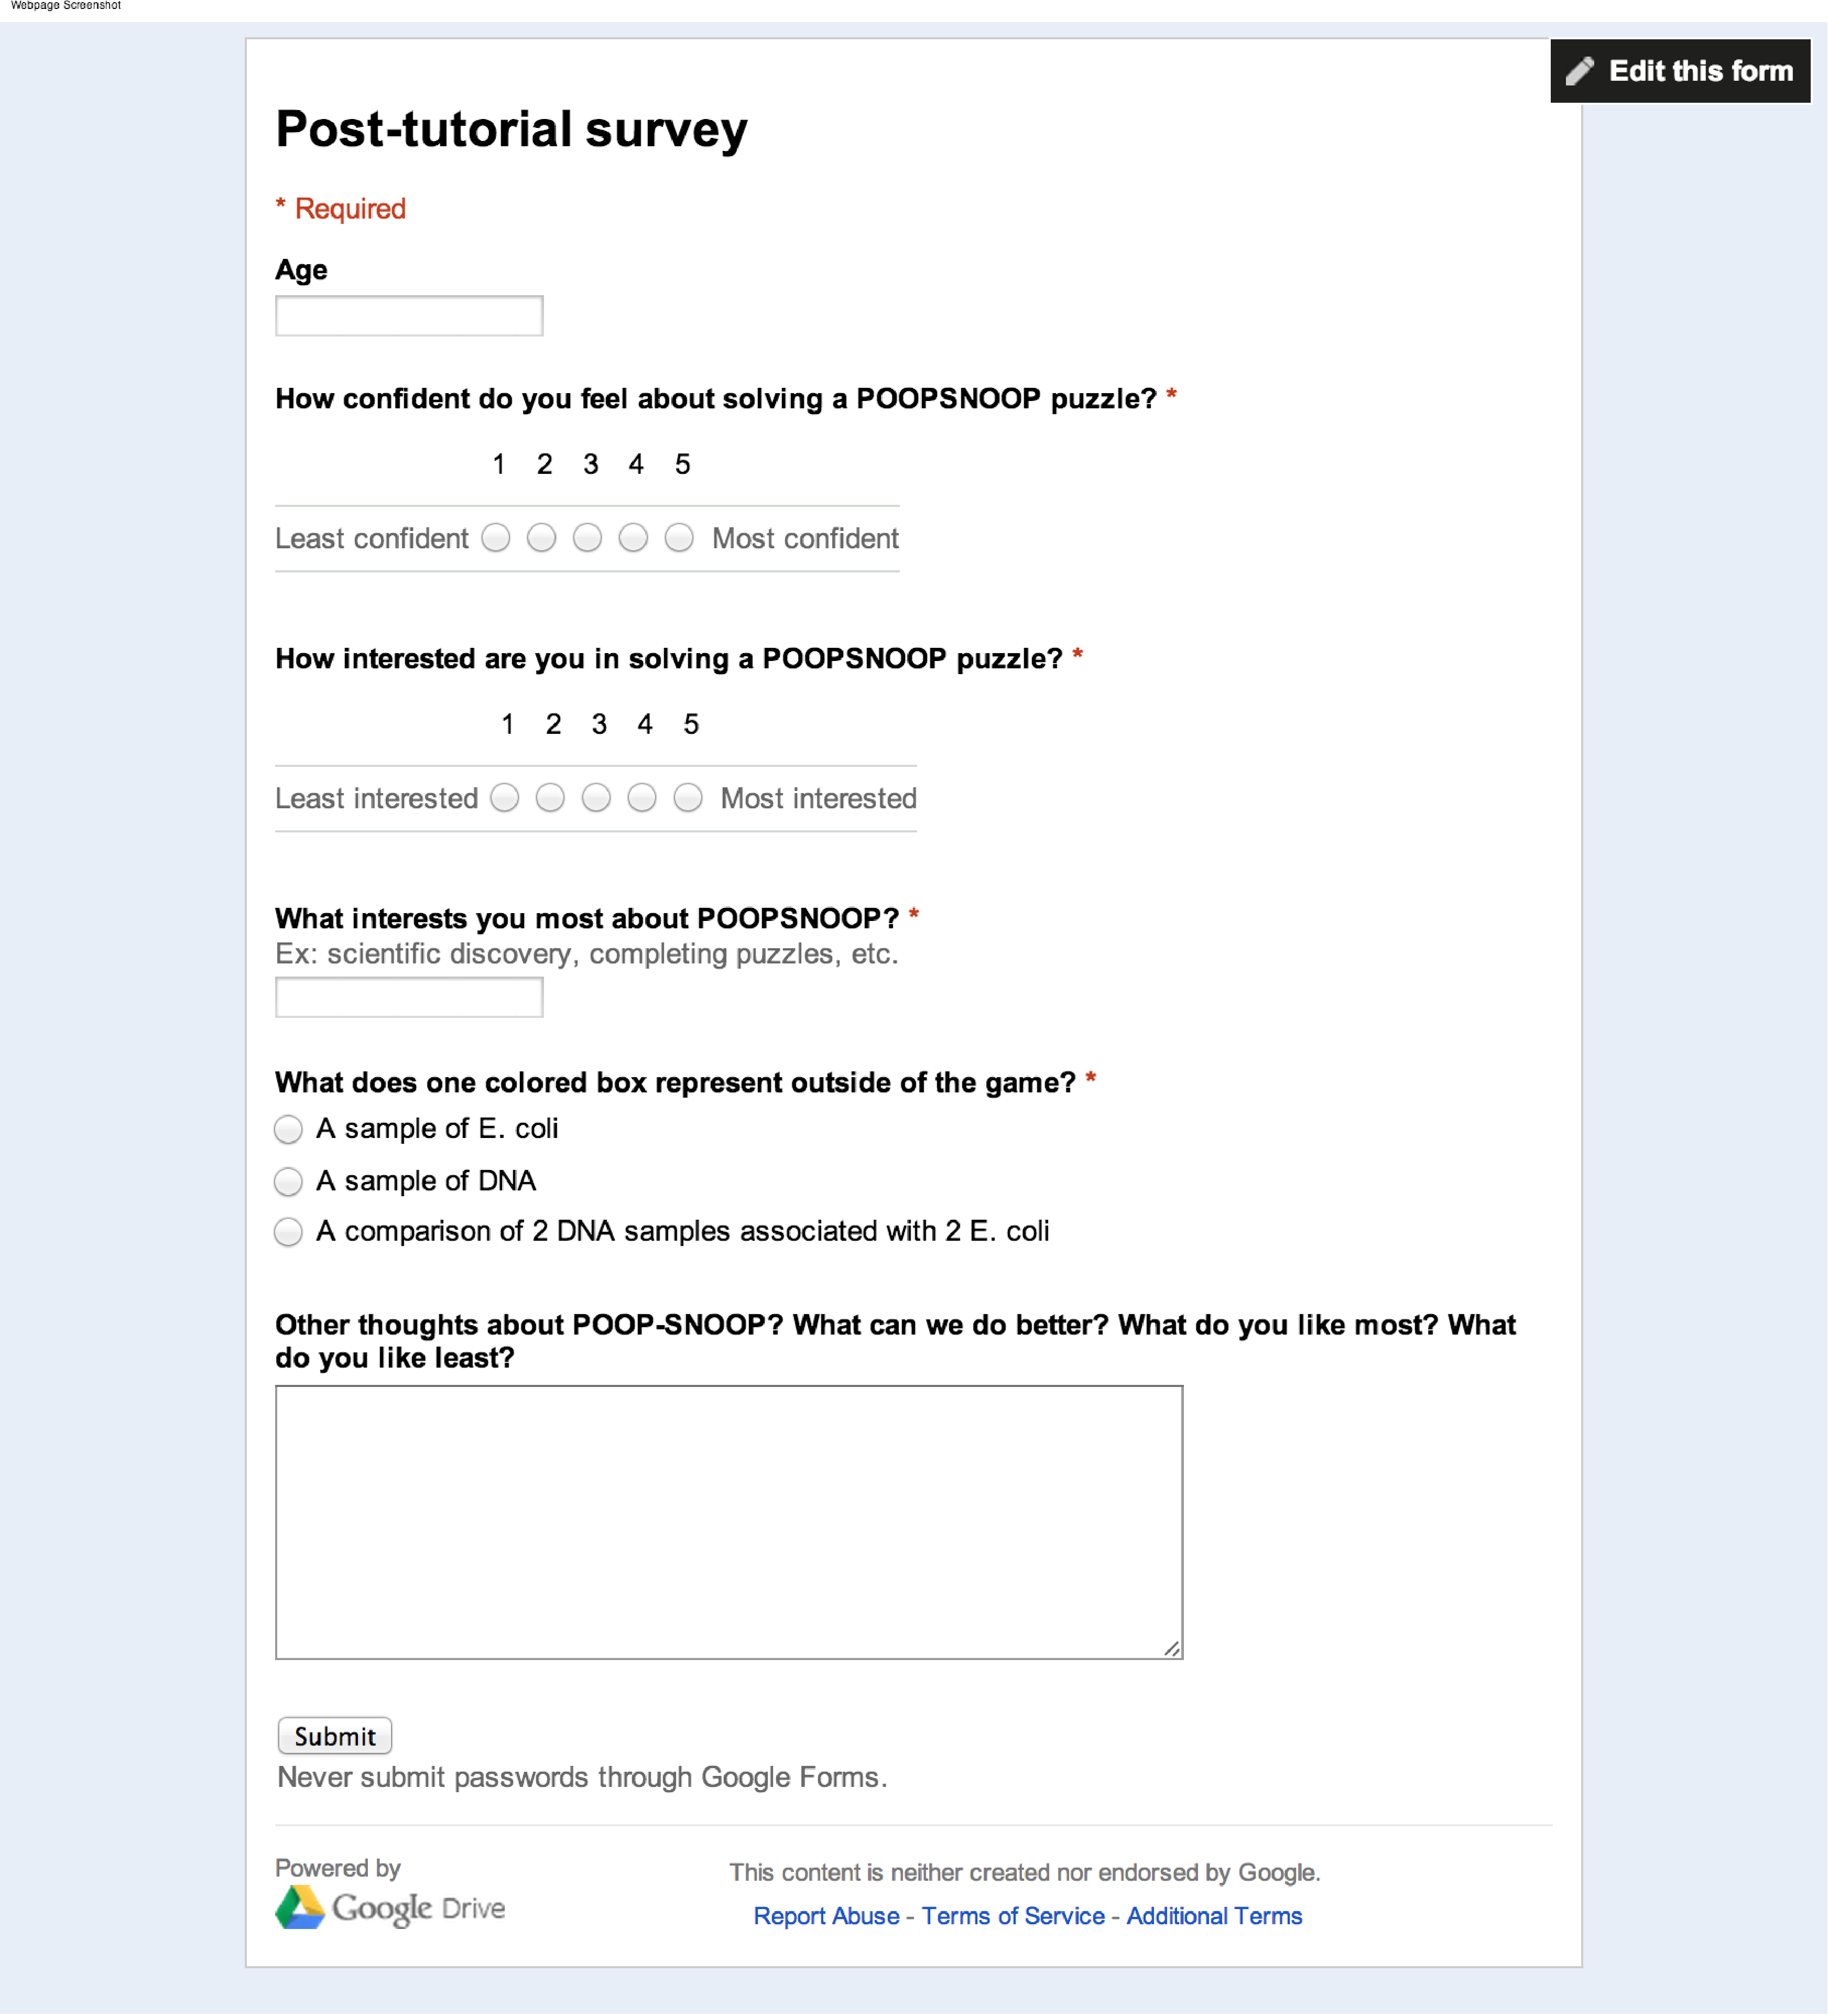
\includegraphics[width=115mm]{images/Post-tutorial.pdf}
   \caption[]{Survey given after the tutorial}
   \end{figure}

   \begin{figure}[H]
   \centering
   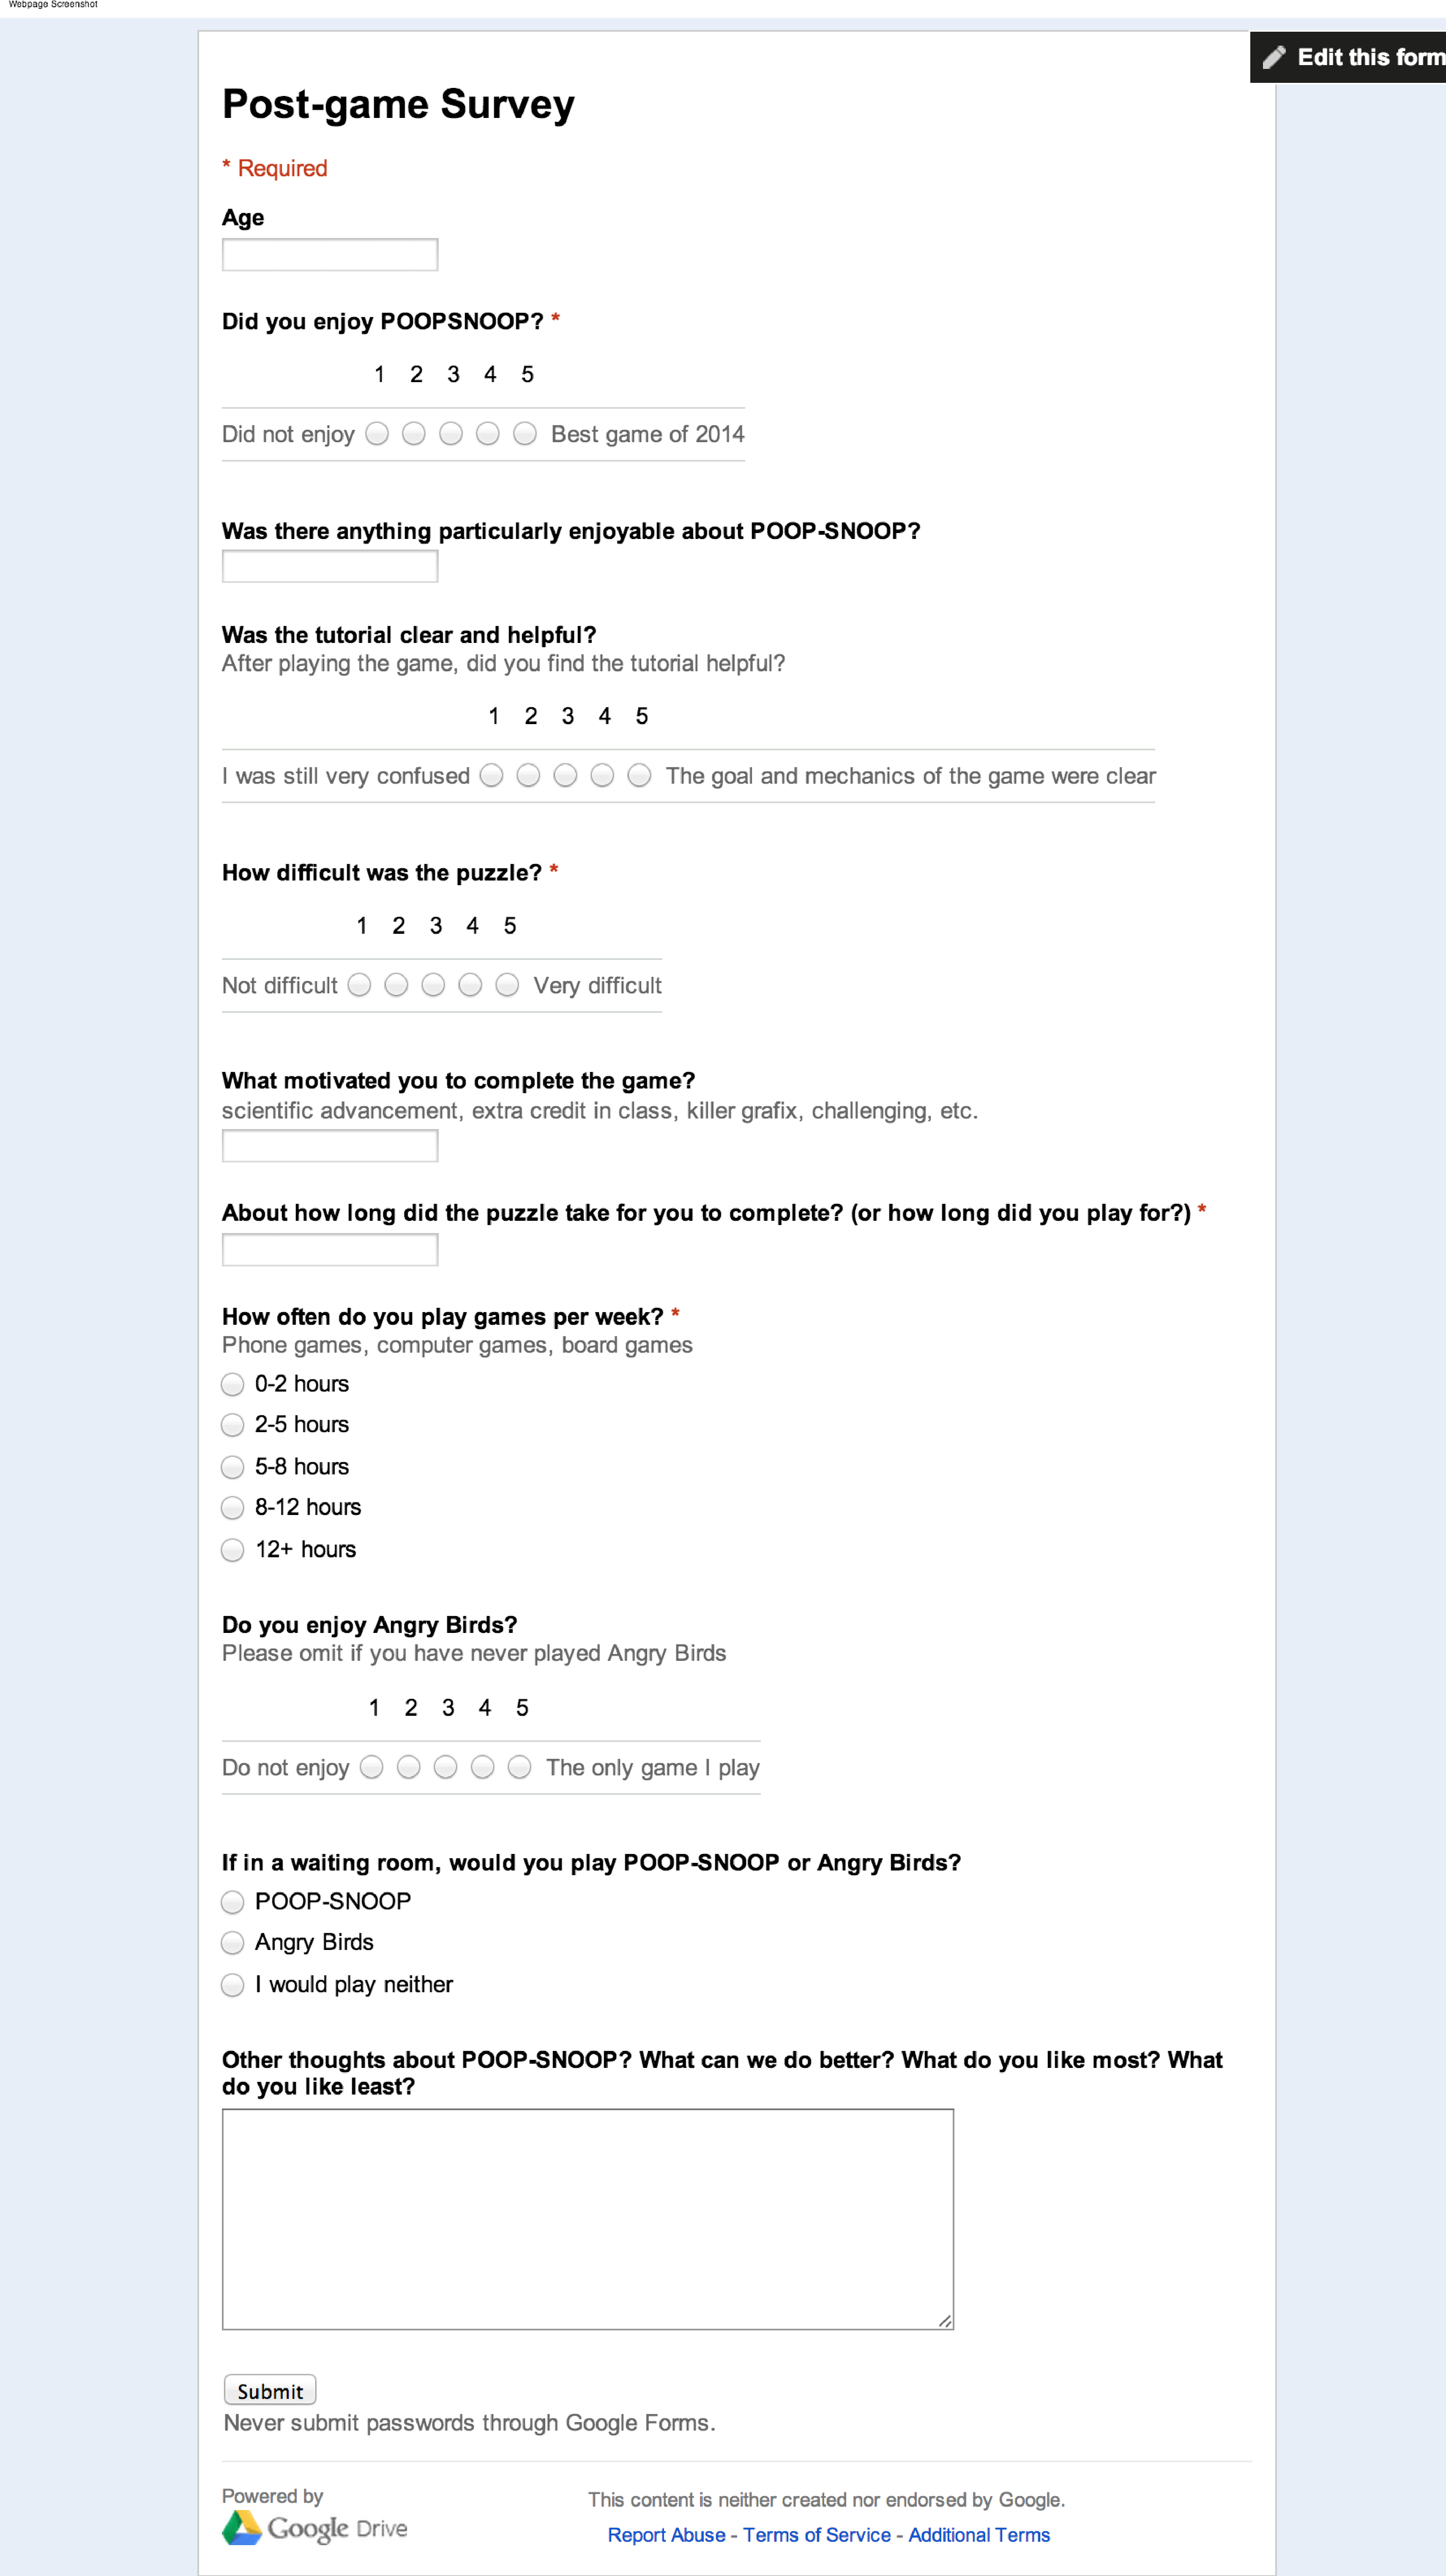
\includegraphics[width=115mm]{images/Post-game.pdf}
   \caption[]{Survey given after the introductory level}
   \end{figure}
}

\end{appendices}

\end{document}
